\documentclass{article}
\usepackage{graphicx} % Required for inserting images
\usepackage[a4paper, total={6in, 8in}]{geometry}  %margins for a4 paper
\usepackage{setspace} %spacing package for words
\usepackage{hyperref} % hyperlinks
\usepackage{cite} %IEEE Cite Format
\usepackage{geometry} %table package
\geometry{a4paper, margin=1in}
\usepackage{array} %table package
\usepackage{longtable}%table package
\usepackage{float}%table and figure ordering
\doublespacing %word spacing 
\pagenumbering{arabic} %add page numbers
\usepackage{amsmath} %math
\usepackage{pdflscape}
\usepackage{pdfpages}


\title{EMAE 398: Capstone Project \\ 
MOHRA: Machined Open-source Humanoid Robot Architecture}
\author{ By: Joshua Huang and Ian Dyke \\ Project Advisor: Dr. Stephen Hostler \\ Project Sponsor: K-Scale Labs (Ben Bolte, Matt Freed, and Paweł Budzianowski )}
\date{December 8, 2024}
\begin{document}

\maketitle

\newpage
\tableofcontents
\newpage



\section{Abstract}

Humanoid robots are emerging from R\&D labs and early-stage companies with the hope of one day assisting us in the home or on the manufacturing floor. These developments have largely occurred behind closed doors, keeping advancement internal to specialized labs and the private sector. To gain insight into the utility of humanoids, these research teams and companies are evaluating their particular designs’ capabilities in various applications. However, the limited options, lack of customization, and high upfront costs of these products hinders such exploration. Opening up development to the growing ecosystem of accessible manufacturing and cooperative engineering (“makers”) allows more individuals to participate in humanoid design and implementation. Enabling broader input will deepen understanding of the mechanical and control requirements of humanoids, raising technical awareness of the challenges associated with designing humanoids and supporting new solutions that advance the field.

We worked with K-Scale Labs to accelerate and open-source a novel humanoid robot design that anyone can build and iterate upon. Our project explores the feasibility of designing a Machined Open-Source Humanoid Robot Architecture (MOHRA) with a focus on efficient weight distribution, machinability, cost, and performance. The MOHRA platform has 23 degrees of freedom and weighs 95 kg. The 6061 Aluminum hardware is manufactured using 3-axis milling tools, water jet cutting, and drilling. The total actuator cost for MOHRA is \$5,800.  MOHRA is a step toward making progress in humanoids more transparent, accessible, and customizable. 


\section{Introduction}

The dream of robotic agents that can do the dull, dirty, and dangerous work in the world has been evaluated through the lens of the human's physical experience. Often we engineer solutions to these issues that do not come close to reflecting the human form factor that was originally performing those tasks. This results in a highly specialized mechanical system that can perform narrowly defined tasks as efficiently as possible, resulting in more throughput, cost reduction, and a higher quality with lower variance. However, these specialized mechanical platforms are rarely capable of translating their skills to a new area without significant effort and time expended to retool, design, test, and validate the mechanical system. Thus, achieving an optimal mechanical design for actions like picking tomatoes or stocking shelves requires the problem space to be well bounded and scoped. However, generalizing the problem to physical space rather than a narrow task results in a spatial manipulation problem that can be applied to an infinite number of tasks. While a mechanical system that has been designed to interact with space will rarely surpass the efficiency of a specialized system, it is capable of performing an infinite number of actions that are only bounded by its interactions in space. Thus, at the tradeoff of specialization, a humanoid robot is capable of navigating spaces designed for humans and executing a wide array of actions in any space. The broad definition of a humanoid is “a nonhuman creature or being with characteristics (such as the ability to walk upright) resembling those of a human” \cite{merriam2024}. The effort required to design one humanoid can rapidly surpass the impact of a specialized machine due to its ability to operate in a limitless number of problem spaces. These advantages are limited by the mechanical capabilities, controls, and internal processing required to exact action in a given physical space. 

A Goldman Sachs research report states that the total addressable market for humanoid robots is projected to reach \$38 billion by 2035 \cite{goldmansachs2024}. The report further cites the maturity of the hardware components and supply chain required for Humanoids has solidified in China while progress in AI research has continued to rapidly advance in the United States. In 2024 more than two dozen Chinese companies released humanoid robot designs thanks to a \$1.4 billion state-backed fund for robotics \cite{li2024}. Humanoid robots present an opportunity to disrupt the current labor market by reducing the cost of labor, improving safety, increasing productivity, addressing labor shortages, and augmenting existing human labor. Disruptive technologies like humanoids also present the possibility of the eventual extinction of many existing labor jobs and the creation of new jobs needed to support humanoid labor. It is impossible to know if the number of jobs eliminated will result in fewer or more jobs being created. Integration of humanoid robots in the labor market will have to be rapidly assessed by regulatory agencies. The human species benefited from spears in the Nomadic age, plows in the Agrarian age, steam engines in the Industrial Revolution, and transistors in the Internet age. Humanoids embody the transition into a new age that will allow us to advance human civilization. 

The state of humanoid robotics has rapidly evolved over the past century. Early research on the study of legged robots was the foundation of humanoid robotic advancements, beginning with the creation of systems capable of performing fixed gait patterns on flat surfaces by individuals like Russian mathematician Chebychev in the 1800s \cite{kim2017}.  In 1962 General Electric unveiled a teleoperated system called the Walking Truck which was “a hydraulically powered, 12 degree of freedom quadruped weighing 1400kg” \cite{kim2017}. The teleoperation of this system quickly became a bridge to the development of automated systems for legged locomotion. In Bekey’s book on Autonomous Robots, he discusses the development of the quadruped system called the “Phoney Poney” in 1968 which “was controlled by a finite-state machine using sensory feedback on the state of its joints, without any internal model of its kinematics or dynamics” \cite{bekey2005}. 

As computers became more prevalent more advanced control systems could be implemented but were challenged when “significant computational resources were required for basic kinematic computations” \cite{kim2017}. To circumvent these constraints mechanical systems were developed with the reduction in computation requirements in mind by Shigeo Hirose in 1984 \cite{kim2017}. The emphasis on exploring mechanisms for legged systems led to the inception of the Waseda Bipedal Humanoid Project in the 1970s \cite{cyberne2012}. Dr. Ichiro Kato led efforts to develop the Wabot 1 which was capable of quasi-dynamic gaits, speaking, and grasping objects \cite{robots2018}. The second iteration built from 1980 to 1984, the Wabot 2 was a more specialized humanoid robot capable of sight reading sheet music, playing the organ keys and pedals, and speech \cite{waseda2024}. These early bipedal machines were limited by their reliance on static stability for balance which resulted in slower movements \cite{kim2017}. 

As Kato continued to push the capabilities of bipedal systems Marc Raibert’s leg lab founded in 1980 emerged as an influential research group investigating legged locomotion when it moved to MIT in 1986 \cite{mit2024}. Raibert’s Leg Lab contributed to active bipedal control improvements, physics simulation models of robots, and various legged robot platforms \cite{mit2024}. Raibert went on to create Boston Dynamics in 1995 which was a spin-out intended to sell robot physics simulation software and consult on robot projects \cite{knight2014}.  Bipedal systems within robotics became a well-established research domain from the 1990s through the early 2000s as passive dynamic walking systems, under-actuated robots, and impedance-controlled actuators were developed \cite{kim2017}. Commercial R\&D efforts to create humanoid robots were also being pursued, most notably the development of Asimo by Honda started in the 1980s and was revealed in 2000 \cite{hays2019}. The humanoid Asimo was capable of walking up stairs, operating on a battery, and kicking a soccer ball \cite{hays2019}. Though impressive in general capabilities Honda ended work on Asimo in 2018 “in favor of working on robots with more practical applications, like robots for elder care and disaster relief” \cite{ackerman2022}.

While Asimo leveraged harmonic drives for operation its novel design paled in comparison to the more functional development of the hydraulically actuated PETMAN by Boston Dynamics. PETMAN was a humanoid robot project funded by the US Army in 2009 capable of walking, running, crawling, and operating in hazardous conditions \cite{guizzo2011}.  Boston Dynamics rapidly advanced bipedal humanoid systems through the US Department of Defense's Advanced Research Projects Agency (DARPA) funded projects and unveiled the Atlas platform in 2013 meant to compete in the DARPA Virtual Robotics Challenge \cite{franzen2013}. The original Atlas robot comprised 28 different hydraulic joints, had impressive balance controls, and an uncanny resemblance to human locomotion \cite{franzen2013}. The Atlas Robot went on to have two additional hydraulic-based actuation generations before it was announced in 2024 that it was retiring its hydraulic platform in favor of an electric-based actuation system \cite{ackerman2024}. Boston Dynamics cited the transition due to focus on commercialization, hydraulic system leakages, and the success of the electric-based quadruped Spot \cite{ackerman2024}. The strategic decision to design robotic systems with reliability in mind while utilizing electric actuators is a clear signal from industrial leaders that robotics is in a transition period that is leaving the nascent stages of development and exploring its applications in commercial settings.

This shift demonstrates the larger transition of humanoid robots from a research problem into a product. Some of the emerging companies making humanoid robots include 1x Technologies, Agility Robotics, Apptronik, Figure AI, Sanctuary AI, Tesla, and Unitree. These companies are in various stages of development. Unitree is one of the first to market selling the Unitree G1 starting at \$16,000 \cite{unitree2016}. Companies like Figure AI and Agility Robotics are beta-testing their early models in customers' warehouses and manufacturing lines in an effort to rapidly iterate their designs. Many of these robots are still under development in company labs and are in a race to reach the market. 

A key limitation of these hardware platforms is their closed development environment. The humanoid robotic domain is still far from a mature market and substantial effort is still required to make these robots into autonomous agents; we could be more than a decade away from such robots folding our laundry or stocking the shelves. A significant constraint to increasing the rate at which humanoid technologies can be improved is accessibility and transparency in both hardware and software. K-Scale Labs is a startup based in Palo Alto, California aiming to make the software and hardware for humanoids open source \cite{yscale2024}. The open-source approach to humanoid development enables anyone interested in the domain to contribute, tinker, and build their own humanoid accelerating the rate at which designs can be iterated upon and the quantity of data that can be collected. Their early designs are focused on 3D printed designs to fabricate their robot Stompy at around a \$10,000 price point. K-Scale Labs is interested in hardware designs that utilize traditional machining techniques to assess the price point, capabilities, and manufacturability of a humanoid for an aluminum-based chassis. Later these designs could be manufactured overseas at scale or by an individual interested in making their own humanoid. In addition, thanks to advances in physics simulation software tools designs for robots can be validated over millions of trials before any parts are put in a CNC mill. MuJoCo and Isaacs are two of the many software stacks that are used to render 3D scenes of the robot and tasks and also simulate the physics associated with joints and actuators, collisions, and material properties that are critical to validating a design. Similar to tools like FEA used for static analysis this will enable us to identify flaws and issues in the hardware throughout the design process. 

The scope of this project is limited to creating CAD models, technical analysis of mechanism functions (ie. torque ratios and output torque), actuator sizing calculations, and a record of the design of mechanical components that make up the humanoid linkages and actuator assemblies. Designed components that make up the humanoid will primarily be made up of aluminum machined using CNC turning or milling as outlined by the project sponsor. It should be noted that other materials and manufacturing methods may be employed if they help achieve the technical requirements and are accessible to the general public. A full bill of materials with approximate costs for off-the-shelf components and a compiled folder of CAD files and drawings will be defined as part of this capstone project. In addition, the defined robot assembly will be trained to walk in physics simulation tools like MuJoCo or Isaac using existing software workflows from K-Scale Labs. The intent is to provide the information and files necessary for a hobbyist or humanoid enthusiast to build or iterate on our design. In addition, we aim to define a design that is lower in cost relative to other humanoid platforms that are available on the platform today to make developments in the field more accessible. 

The company K-Scale Labs has defined the power system, electronics, software, and actuators that will be used as a starting point for the design. The fabrication and manufacturing of the complete humanoid was deemed out of the scope of this capstone project. In addition, developing software, electronics, supply chains, marketing, and business development are all out of scope for this capstone project. The capstone team does have direct communication with both Ben and Matt from K-Scale Labs over Discord to review and advise on technical decisions. In addition, the faculty advisor, Dr. Hostler will advise on the overall project direction and consult on the progress of the project and achieving defined deliverables of the capstone project. 

%%%%%%%%%%%%%%%%%%%%%%%%%%%%%

\section{Design Approach}

At the outset, the development of the MOHRA humanoid was split into a few key design steps and cycles. These are:

1) Research and Ideation

2) Draft Model and Simulation

3) Performance Review and Design Definition

4) Prototype Design and Simulation

5) Revision and Continued Prototyping


The intent of this project flow was to enable an initial familiarity with the design tools and existing knowledge of the design of humanoid robotics. This supported the team as we moved into the heavily iterative process of design, review, and revision required for developing the complicated and interdependent systems that make up a humanoid.

\subsection{Research and Ideation}

Being a field that is still new, the understanding of legged robotics and especially humanoids is heavily centralized in a handful of major private companies and research labs. There is significant diversity in the approaches taken in developing each system, and at this point, many of the implementations are still intent on pushing the field forward, rather than moving into standardization and mass production (it is only now that we are seeing major efforts in implementing these sorts of robots into working applications \cite{unitree2016} \cite{agilityProducts}). The publications coming out of the research labs have done well to document the key takeaways and principles discovered throughout their project. On the other hand, while the private groups do not publish their specific design process, they do often provide performance data and videos on their designs. Comparing these peers in the market, in their build choices and the corresponding performance, also provides a wealth of useful insights into humanoid design. There are a few universal 'rules of thumb' one can see in all of these resources, but for the most part, each implementation brings its unique understandings that build on the previous peers in the field.

To develop our intuitions, we spent a significant portion of the project (about 30-40\% of our time) pursuing different research papers -- the theses being especially useful -- and aggregating information on the different specifications, joint layouts, and capabilities of robots now on the market. These formed a basis of knowledge that allowed us to steer subsequent design and development effectively, giving insights into critical metrics, useful design philosophies, and pitfalls to be avoided.
The following subsections describe some of these takeaways:

\subsubsection{Body Dynamics}

Much in the way weight impacts the suspension on a car, the flight of an airplane, or the control of a rocket, mass distribution in legged robotics has an out-sized influence on the capabilities of the machine -- from energy consumption to outright dynamic performance. Due to the compound linkage needed to create an arm or leg, this effect is multiplied further, making the extremities the major challenge in all humanoid designs. In general, the desire is to minimize the weight of all components, and more specifically to minimize the effective mass moment of all appendages as relative to the trunk -- where the trunk itself is kept on a linear path through the walking gait to reduce its inertial effects. This allows the robot to move more quickly, with faster reflexes, and with less energy consumption.

%The dynamics of the robot are further impacted by the 'mechanical impedance' of the body, which describes the motion in terms of the aforementioned inertia as well as the stiffness and damping within the structural elements. (( To be continued -- need to do more research on this as we begin applying it )).

\subsubsection{Actuators and Motors}

The motors within the robot are the major constraint on limiting weight in the extremities. Historically, it has been seen that "the actuators typically compose up to forty percent of robot mass" [McKenzie, 2012, p. 59], and they necessarily must be placed somewhere on the arm or leg. As such, the intent is generally to implement the lightest motor assembly possible to achieve the needed forces and velocities.

In consideration here are the thermals of the motor -- making sure that it does not destroy itself from the load, especially given the need to push the smallest motor possible to its maximum capabilities. However, in the heavily fluctuating and often intermittent loading conditions of the arms and legs, thermal/power ratings of the motors for continuous output are not well-reflective of the performance of the motor in application; they can be seen more as a conservative 'proof' value for establishing static body states and load-carry capacity. The capabilities of motors past this rated load/voltage/thermal specification are rather uncertain. Many companies offer a 'peak' value alongside the 'rated' value, but there is a clear difference either in how companies measure or how well the internals can operate between these two regimes: the peak is generally at least double the rated, but then may vary from 2x up to 6x depending on the company, model, and integrated transmission (see \textit{Appendix D, Motor Market Analysis}). It seems that truly reliable evaluation of motor performance and optimization is reliant on empirically testing the motors, as was done by Katz \cite{katz_low_2018}.

With this in mind, the majority of legged robotic motors have moved to utilizing large gap-diameter motors, moving the hobbyist/prototyping space into using "high performance brushless motors [intended] for RC drones and airplanes” \cite{katz_low_2018} % (Katz, 2018, p. 23). 
These present an ability to output relatively large amounts of torque (due to the large diameter of the windings) without needing to rely on a large gearing reduction; generally speaking, they're only coupled with a single-stage planetary gearbox (and thus limited to about 1:10 reduction). This motor configuration, being as close as possible to direct-drive motors, is thus named 'quasi-direct-drive'.

These motors present various advantages in their layout and performance compared to traditional high-rpm high-reduction motors. Their high torque relative to weight is necessarily useful \cite{katz_low_2018}; %(Katz, 2018, p. 23)
their wide-but-thin packaging generally is better suited to being mounted on limbs; and their ability to spin at slower speeds limits inertial effects and drag losses within the system. This last point is generally the major advantage for quasi-direct drives, providing a "transparency" \cite{seok_actuator_2012} %(Seok et al., 2012, p. 1970)
in controlling the motors by eliminating the transient effects one would see with a fast-spinning gearset. In fact, in many cases it is possible to utilize the electrical feedback of the forces on the motor to inform the control system (in lieu of a strain gauge in the linkage, or similar) due to the backdriveability of these motors. \cite{katz_low_2018} %%<< CITE ME -- Katz? >>


As a final note, the usage of these motors also creates a larger footprint for the housing itself, allowing it to be designed as a structural element within the larger structure of the linkage; this provides a more versatile means of integrating the motor into the rest of the assembly, and "reduces total mass and often increases strength. \cite{mckenzie_design_2012} % (McKenzie, 2012, p. 59).

\subsubsection{Joints and Linkages}

The most basic performance metric of any humanoid robot is the Degrees of Freedom, detailing the number of ways the robot may pivot, slide, or otherwise translate its components relative to each other. Fundamentally, the desire is to emulate a human body; however, the fact that human joints are actuated by an unquantifiable number of muscle fibers, with motion able to be "produced in an infinite number of ways” \cite{mizrahi_mechanical_2015} %(Mizrahi, 2015, p. 1) 
by activating different groupings of them, makes a direct emulation approach unfeasible at this time. With the limits of packaging rotary motors and linear actuators in mind, joints on humanoids typically rely on simple pinned pivots and coaxial-driven pieces to emulate the extension/retraction and twisting motions of human arms and legs. More complex linkage systems are invoked when specific motion characteristics are required, but also necessarily provide a more limited range of motion. One will generally see that the humanoid robots have fewer degrees of freedom than real humans -- forgoing the ability to twist (roll) the shin after the knee, as an example. Instead, they rely on larger ranges of motion in their joints to still achieve a similar overall movement capability. Traditional robot and control designs rely on a fully defined system where each degree of freedom of the system can be controlled by an actuator. Legged robots are dynamic by function and are not fixed to a datum as they traverse through space. A humanoid robot can actuate all of its mechanical degrees of freedom as well as six additional degrees of freedom that define its position and rotation in space \cite{underactuatedruss}. 

Once the degrees of freedom are laid out, the choice of interconnection between the motors and the chosen joints has direct implications for the mass distribution in the robot. Following the principle of lowering the mass-moment of the limbs, it is advantageous to move motors closer internally to the body wherever possible. A common choice now is to see the knee pitch (extension) be done by a belted transmission rather than directly by a motor; the added complexity is made up for by allowing for the motor to be moved into the upper leg next to the hip, closer to the trunk. Such a trade-off can be seen in the Adam Robot by PNDBotics \cite{pndboticsAdam}.By shifting the hip motors for leg actuation closer to the hips center of mass this also increases the legs range of motion during walking strides. The Figure 01 robot and Tesla Optimus robot walking gaits were very short and contained significant movement in the hips during movement that would result in additional actuator movement and thus additional energy expenditure. Further, the motors must be tailored to the joint -- smaller, less massive motors for less stressed joints. Katz notes this for quadruped legs, using biological data as justification that “a stronger elbow actuator may be placed in series after a weaker shoulder actuator without jeopardizing the dynamic performance.” \cite{mckenzie_design_2012} %(McKenzie, 2012, p. 58) 
Tailoring the motors to the joint, and the joints to the motor will allow for mass-moment to be decreased overall.

An interesting approach in building the joint for the motor is using linkage systems rather than standard transmissions. A prime candidate for this is the ankle, where there is simultaneously a large amount of load going through the joint and a relatively limited need in range of motion. Instead of relying on a direct motor connection, it is possible to use a bearing connection (a combination of pitch and roll bearings, a cardan joint, a ball and cup joint, etc.) with a connecting rod joining it to a distantly-placed motor to form a linkage similar to an Achilles tendon. The bearing will accept a portion of the static load of holding up the robot, and the design of the linkage provides more mechanical advantage to the motor. Doing this allows for, once again, smaller motors located closer to the trunk; a good example of this is the PNDBotics Adam \cite{pndboticsAdam}, among others. In general, it is advantageous to implement linkages where constraints allow and designing geometries to focus static loads into the joint structure rather than into the motors.

\subsection{Draft Model and Simulation}

Components within battery-powered robots are heavily interdependent, which means designing components with isolated requirements and considerations will not result in a successful design. As Katz states, “No individual element stands on its own... when one component changes, the remaining elements must be reevaluated and refined iteratively.” \cite{mckenzie_design_2012}%(McKenzie, 2012, p. 45). 
As such, the most efficient first step in developing the design of a humanoid is generally to start with a bare-bones model of the overall form. This 'first draft' is intended to prove the basic capability of the robot to move itself, develop initial values for joint loads and power requirements, and catch any glaring issues in what the designer has in mind for their design.

At the outset, the goal is to develop some initial ideas on performance characteristics desired out of the robot. The 'intangibles' of the expected end product -- what it is meant to do, what actions it should be able to do at what speed, etc. -- are important to lay out initially, and turned into specific metrics and values that the robot will be built around. With these \textit{performance metrics}/requirements in mind, it is then also useful to develop a set of \textit{design metrics} that are more directly related to the components and more directly measurable in simulation/testing. For humanoids, some common metrics in this domain are Cost of Transport relating mobility to the power required to enact it; Gait Tracking, seeing the vertical travel of the hip/trunk during walking; %a secret third thing.
These should have a certain range of values associated, but are more flexible than the performance metrics, being focused on enabling the design to trend towards the performance metrics rather than being an end in themselves. Finally, turning these metrics into specific draft design values, informed by peers and existing literature, will give a good sense of what the robot should look like.  All this is done to facilitate decisions on, at minimum, the robot's degrees of freedom, joint layout, and general mass distribution -- the 'skeleton' of the robot.

To clarify this further, a decent analogy can be made with a combustion car engine. With a nebulous idea of producing a 'gas-efficient' engine for the consumer, the designer first quantifies what 'gas-efficient' actually is - say 30 miles per gallon, looking at peers in the market. From there, there needs to be an understanding of what factors go into enabling this fuel economy. Research would show that there are some design metrics already understood for good engine design, quantities like Compression Ratio, Air/Fuel Ratio, various valve timing and airflow needs, among others. Assigning specific values or ranges to these metrics will then allow the designer to make informed decisions on the mechanical elements and layout of the engine. There will still be iteration as one begins building out the model for the engine, but this approach will narrow in the range of likely options for the components and provide metrics to test against earlier in the design, speeding up and simplifying the process.

% I don't like this... continue on
Returning to humanoids, having this skeleton of the robot defined is useful to simulate its performance capabilities in a physical environment. Running a physics engine, assigning joint types and ranges of motion to different components, and providing the rigid-body 3-D model 'agent' with some basic control system/learning model to guide it into useful motion, the humanoid design will begin showing its strengths and weaknesses. At this point, the goal is to have the robot perform some of the basic tasks from the performance metrics, and to analyze the design metrics that correlate to these. It will likely be heavily iterative, but the simplicity of the draft model skeleton is intended to make changes and simulations quick to solve.

Another benefit of this approach is getting familiar with the model-to-simulation workflow early on. Current progress in humanoids has been useful in the development and distribution of the physics engines as well as various interoperability capabilities for importing updated models and implementing the control/reinforcement learning systems. Open-source/freely distributed simulation environments (Mujoco, Isaac Gym/Lab);
popularized standard filetypes for robot definition (URDF);
API-integrated import/export capabilities for 3D models (\href{https://github.com/kscalelabs/onshape}{k-scale KOL for OnShape}) \cite{kscalelabsonshape_2024}; % cite me, and another?
streamlined training routines (\href{https://github.com/kscalelabs/sim}{k-scale sim for Mujoco}) \cite{kscalelabssim_2024}; % cite me proper, and another?
all of these now exist to decrease the friction of starting up and iteratively improving humanoids. Setting up these workflows early on benefits the project later into the cycle when the focus is better spent on more specific design issues and optimizations.

\subsection{Performance Review and Design Definition}

With the skeleton developed to a functional level, the next step is review of the design metrics. Some of these (standing stability, walking gait) may have been found through the simulations; others, like analysis of mechanical impedance characteristics, may need standalone calculations. This review is done to assess how well the current robot fits the previously defined design metrics and how well the design metrics themselves predict the performance of the draft model. There may be opportunities to refine the design metrics to better fit the desired performance based on the data; some metrics may not reflect the requirements for the given task; or there may be new opportunities to define alternative metrics. It may even give cause to return to the original scope of the project if it becomes apparent that there will need to be trade-offs between the performance metrics. In any case, this is the ideal point at which one lays out a more informed testing/validation procedure before moving into the full iterative design cycle.

Further, this is the point at which it is useful to begin defining reasonable limits to the physical systems of the robot. The force/torque and power/energy data found in (or able to be derived from) the previous simulations will be essential in specifying the materials needed. Establishing what available motors, actuators, encoders, bearings, batteries, etc. may be used is an immediate necessity for establishing \textit{real} design values. Determining what materials may be capable of carrying the loads expected will give a better sense of costs, both in raw stock and processing/machining. It may become apparent custom solutions will be needed, as was the case for Katz in creating custom motor housings and gearboxes. \cite{katz_low_2018}
These are all essential aspects of honing in on the final design, and getting them out of the way as early as possible is advantageous.

\subsection{Prototype Design and Simulation}

The Prototyping phase is where the development of a realistic model for the humanoid begins. Informed by the research and analysis up to this point, with a good sense of the general 'skeleton' of the robot and how it can be adjusted, and an initial list of what materials may be incorporated into the design, the focus turns to integration and optimization. Fitting the motors and associated hardware and power trains within each limb is the first challenge. Then, using the required interfacing points and the load data from the simulations, the structural elements can be intelligently designed -- with additional possibilities of leveraging finite element analysis (FEA) and, possibly, topological optimization (TopOpt). Gradually coordinating all of the different elements will eventually lead back to a functional humanoid robot model.

This functional model will then be passed through the established model-to-sim pipeline to determine its performance against the idealized draft model. Ideally, it will perform similarly well, though it also may require re-evaluating the mass distribution and structural layout of the system. Once the robot is shown to be capable of the fundamental mobility required of it, there is also the opportunity for building out the simulation environments and conditions to further stress and challenge the design; it will be useful to establish some realistic values for loads, response time, etc. during 'edge cases' that the robot may see in reality. 

\subsection{Revision and Continuous Prototyping}

From this point, it is a matter of iteratively re-designing and simulating the humanoid's performance, gradually approaching the intended performance requirements and optimizing wherever possible. Most of the workflows will be established. As such, the designer or team's attention can be focused almost entirely on reviewing performance, brainstorming improvements, and coordinating the knock-on effects of each individual change. By establishing the initial knowledge and experience base as described through this approach, this portion -- the most difficult from a strictly engineering standpoint -- should be made more straightforward and quick-turnaround as the design is brought to a truly functional state.

In terms of the MOHRA team's implementation of this process, the time limitations on the project are likely to prevent us from establishing a fully optimized final design for the whole robot. As such, the intent is to work through at least one, and ideally two, of these prototype-revision cycles. Our focus is primarily on improving and optimizing the lower body of the robot. We see these choices in scope as the most efficient way of developing a 'platform' of a robot for usage in K-Scale's open-source project; the goal is to establish a design for others to build off of and iterate with themselves, so the initial high-friction, low-information steps are our primary concern in development and documentation.

\subsection{Joint Layout and Humanoid Design}
%Joint Layout and Overall Humanoid Design
To design a humanoid we started by determining the layout of our joints and linkages. Out of the options of revolute, prismatic, and spherical joints, in our system, we used revolute joints in our humanoid since we designed for bipedal motion in our system and wanted to represent our degrees of freedom about defined rotational points. In addition, the actuator designs for revolute systems can be purchased off-the-shelf and can be mounted in place to output torque. This increases the simplicity of design and reduces the complexity of installation, design, and control of the completed humanoid system. The next issue we worked through was defining the number of degrees of freedom we wanted our system to have. We reviewed a wide range of current and previous humanoid robot designs from Agility Robot, UCLA Artemis, Unitree G1, Tesla Optimus, Boston Dynamics Petman and Atlas, PNDBotics, Xpeng, Honda Asimo, Stompy and Stompy Mini, Booster T1, and Figure 01. After reviewing these designs we noticed that actuators were not always placed directly at the point of rotation, walking gaits were highly variable based on the design of the hip, and that adding additional degrees of freedom did not always equate to a more capable system. These humanoids also helped determine where and how many actuators would be necessary to perform actions like walking or manipulating objects. We started by outlining the location of joints as well as the number of linkages. From there we parameterized these components to adjust the length of each linkage and the placement of joints in the arms and legs. This defined the skeleton of our system we would design around. Finally, we considered the axis that each joint would be rotating about. In the arm design, we opted to go for a design where each rotational axis was perpendicular to the previous one. But, in the hip and leg design, we decided that the joint for leg swing actuation would not necessarily be perpendicular to the previous joint since the method in which the hardware is mounted and the location of the pivot point relative to the center of mass of the hip would influence how much energy would be expended during each step. 

\subsection{Moment Calculations and Actuator Loads}
To transition a design from a hardware layout into a mechanical design, there must first be an understanding of what the torque loads will be on each joint since this will determine the rated torque load requirements for the actuator that will be chosen for the joint. Some key assumptions needed to be made about the geometry and mass of each linkage in order to define preliminary masses and thus static loads that each joint could be expected to sustain loads under. For the arms, cylindrical tubing with a defined wall thickness, outer diameter, and length was used to determine the volume of material. The volume was multiplied by the density of our material which was 6061 Aluminum in order to define the mass of each arm linkage. Now that the mass of each linkage was defined and the position of each pivot point was also defined it was possible to determine the moment load that each joint would need to sustain. The mass of distal joints was treated as a point mass and estimated mass values were input in order to account for all loads that the pivot point would experience. The total moment at each actuator was calculated using equation 1. In addition, for the leg layout I beams were selected since the leg linkage loads were under bending loads that were not axially compressive at all times. This meant that the I beam was more mass efficient for sustaining bending loads compared to a tube or square tube hardware structure which was critical to reducing overall leg mass. An I beam CAD model was loaded into OnShape and parameterized to the number of linkages in the leg and hip. The mass properties for 6061 Aluminum were used and the mass was determined for each linkage. The placement of joints and mass of joints was also approximated in the OnShape assembly in order to determine the range of motion of the leg as well as determine the position of the joints. The mass and length values were then recorded and the joint torque loads were calculated using equation 1. Finally the knee actuators static knee load based on pivot was not the maximum load case. The maximum load case for the knee was defined as the squat position of the knee and the total mass of the upper body. The knee joint would pivot about the knee in order to resist the moment created by the upper body based on the bend angle of the knee. This dicated the highest rated torque load case that we needed to specify an actuator for. 

%\begin{equation}
\begin{align}
    M_{\text{pivot}} = \sum_{i=1}^{n} \mathbf{r}_i \times m_i \mathbf{g}_i + \sum_{j=1}^{m} \mathbf{r}_j \times m_j \mathbf{g}_j
\end{align}

\begin{itemize}
    \item $M_{\text{pivot}}$ — Total moment about the pivot point.
    \item $\mathbf{r}_i$ — Position vector from the pivot point to the location of actuator $i$.
    \item $m_i$ — Mass of actuator $i$.
    \item $\mathbf{g}_i$ — Gravitational acceleration vector at the position of actuator $i$.
    \item $\mathbf{r}_j$ — Position vector from the pivot point to the center of mass of linkage $j$.
    \item $m_j$ — Mass of linkage $j$.
    \item $\mathbf{g}_j$ — Gravitational acceleration vector at the center of mass of linkage $j$.
    \item $n$ — Total number of actuators.
    \item $m$ — Total number of linkages.
\end{itemize}

\noindent \textbf{Explanation:} \\
The total moment $M_{\text{pivot}}$ is the sum of two contributions: 
\begin{itemize}
    \item The moment caused by each of the $n$ actuator masses, where each actuator of mass $m_i$ is located at a distance $\mathbf{r}_i$ from the pivot. The force on each actuator due to gravity is $m_i \mathbf{g}_i$, and its contribution to the moment is the cross product $\mathbf{r}_i \times m_i \mathbf{g}_i$. 
    \item The moment caused by each of the $m$ linkages, where the center of mass of each linkage $j$ is located at distance $\mathbf{r}_j$ from the pivot. The gravitational force acting on the linkage of mass $m_j$ is $m_j \mathbf{g}_j$, and its contribution to the moment is $\mathbf{r}_j \times m_j \mathbf{g}_j$. 
\end{itemize}

At each joint, the total moment on it was determined in order to define a minimum specification for the torque load that an actuator would need to be capable of actuating to be functional. The mass approximations for each linkage and joint were biased to slightly overestimate the mass of the hardware components to ensure that actuators would not need to be re-specified. In the event that they would need to be re-specified, we created a torque calculator so we could parameterize and update the torque loads on each joint based on the hardware design. 

\subsection{Actuator Specification and Cost}
%Actuator Specification and Cost 
Now that each joint's maximum moment load case has been defined it is possible to specify the actuator hardware that is necessary at each joint. Typical motor specifications list multiple parameters like peak torque output and rated torque output. We chose to specify motors to the rated torque output rather than the peak torque output since our max moment load cases calculated were in the bounds of loads that the actuators would be expected to sustain continually. If we specified our actuators to the peak torque of an actuator the hardware would only have been capable of maintaining that load for a short period of time, would require additional voltage draw, increase wear on batteries, and also result in overheating of actuators. The key function of the actuator is to convert electric energy into rotational torque. The planetary gear actuator architecture is made up of a stator, rotor and output shaft, and gearbox. The stator is a coil of copper wire that is wrapped in a defined pattern in order to create a magnetic field when current is run through it. The rotor and output shaft are placed in the center of the stators magnetic field and the magnets on the rotor interact with the magnetic field in order to create rotational torque which is output by the output shaft. The output shaft can then be connected to various gearbox mechanisms in order to create defined gearing ratios for desired torque output while controlling the rotations of the shaft per minute or the speed of rotation. Various gearbox systems were considered including harmonic drives, cyclodidal drives, and planetary gears offered by suppliers primarily out of China. We chose a planetary gear system for our actuators since it had lower gear ratios which meant we could maintain high torque bandwidth and torque output compared to a harmonic drive or cycloidal drive which gear down the RPMs of the output torque. 

The overall mass of the actuators was also a key consideration will selecting actuators. We desired that the packaging of the system was lighter since it would reduce the overall mass of the hardware and reduce the required rated torque of the hardware and this was especially true at the distal joints on the limbs. A key observation was that as the actuator packaging at the same torque output had an overall mass reduction due to packaging design the cost of the hardware increased significantly. The Robstride actuators we opted to specify for our system were almost twice the weight of the equivalent MyActuator offering but the Robstride actuators were half the price. The maximum axial load of the actuators was also a key consideration. It became clear during the market search for actuators that we would need to pursue specifications on the maximum load that the actuator could sustain to make sure it would not fail under its own weight. The Robstride actuators as well as other actuators axial load ratings were almost an order of magnitude higher than our requirements. Actuator communication and control protocols were also a key consideration. From an electronics stand point standardizing the communication standard and commands sent to various actuators would ensure that later controls work would be more simple. Various communication protocols varied based on the motor control boards that were installed on the actuators and included Ethernet, CAN Bus, ESP32, and RS232. The key here was to ensure that all the actuators we selected were on the same communication protocol. For our purposes we selected the CAN BUS protocol provided Robstride since it also had supported packages created by K-Scale. 

Back drivability of actuators was also a mechanical aspect we wanted to ensure our actuators were capable of. In the event of a safety issue where the actuators move joints, we wanted our mechanisms to be able to be moved by a human or external force in order to adjust the angles of actuators. Thus, we selected actuators with defined back drivability as well as defined torque required to back-drive them. This meant if the actuators were not energized they could still be moved in safety scenarios. The actuator speed rating in RPMs was also considered. Since humanoids are performing dynamic tasks like walking or handling additional external loads, actuators that make it up also need to be capable of moving quickly in order to adapt to constantly changing external loads. We biased toward selecting actuators that were at a minimum more than 100 RPM and if there were too similar actuators in cost and rated torque we would select it based on the higher RPM specification. Encoders were also something we considered when selecting actuators. At a minimum we wanted our actuators to be dual encoded to be reliable and increase fault tolerance in the event that an actuator was not performing properly it would be possible to identify the drift in positional accuracy. Actuator backlash was not a key specification but could be considered in the event that actuator precision is a requirement based on the tolerances for joint movement accuracy. Finally, the actuators mounting system was considered and most had rear face or front face tapped holes that could be used for mounting to static hardware as well as mounting the torque output. If actuators did not have defined mounting points already defined we decided not to consider them due to the risk of modifications to actuator hardware without validating it ourselves first. 

The overall approach for selecting motors was to place them at the joint location where possible. For the knee joint based on the rated torque load requirement calculations, it became clear that if we specified an actuator that would be placed at the knee directly based on the rated torque requirements of 85Nm we would be spending upwards of \$2,000 per a knee actuator. This was far above a reasonable spending goal since most actuators were to cost \$300 and we noted that this actuator would require a mechanism in order to achieve an output torque that met rated torque requirements. In other instances like at the ankle, we wanted to minimize the amount of mass that was at the distal end of the leg and placing actuators at the ankles would increase the moment required per step of the humanoid. To counter this we decided that the actuators would need to be placed higher in order to reduce the moment, but this would require that the torque would need to be delivered via a designed mechanism. To review the actuators that were considered in depth refer to appendix D. 


\subsection{Mechanism Selection and Design}
%Mechanism Selection and Design
The key mechanisms we needed to design were for the torque at the knee and at the ankle. The knee mechanism needed to sustain high torque loads and be reasonably light due to the already high mass of the femurs structure. It also could not reduce the torque bandwidth of the input actuator to the point that the knee was slower than 100 RPM. We considered various mechanisms including chain drives, belt drives, ball screw transmissions, capstan drives, and rolling joint mechanisms. Out of all of these options the belt drive was the most compelling as our mechanism of choice for knee joint torque transmission. The chain drive was very heavy which meant our moment would increase. The ball screw transmission had a higher number of parts and lowered the output rpm of the knee joint. The capstan drive was a compelling choice and was considered but due to the manufacturing and assembly complexity we decided against. There was a risk of high variance in tension between capstan drives which would directly effect the control system that the drive system required and would increase variance in control profiles between knee joints. The rolling joint mechanism was the most similar to an anatomically accurate knee joint, but also came with all of the constraints and hardware considerations required to imitate that anatomy. The knee had a more limited range of motion and required additional tendon like drives in the femur in order to actuate it. In addition, the means of control over the knee joint was less defined relative to an actuated torque output and we would need to map the linear displacement of the linear tendon to joint actuation overall increasing the complexity of the knee design. Finally the belt drive was the most feasible due to its low complexity in hardware design and control profile. The output torque of the actuator would simply need to be converted based on the output pulleys torque ratio. The main considerations were for assembly clearness for the pulley wheels and belt and the tensioning of the pulley during operation. We opted for tensioning system that would engage the belt with bearings and constrained widths. A spring tensioning system was considered but would increase complexity since it would need to maintain tension if the direction of rotation was invested. A key tradeoff of the belt system was a reduction in the knee joints stiffness since the belt was now maintaining the position of the knee angle. For future revisions placing an encoder at the knee joint output pulley may be useful to improve the knee joint if the control profile has significant drift. 

The ankle joint actuation about its pitch and roll axis was enabled using a universal joint mechanism retained by cir-clips. The pitch and roll actuators were shifted toward the top of the tibia in order to reduce the moment. To deliver the torque to the ankle we adopted a 4 bar linkage system for both the pitch and roll. Based on our market research if actuators were not placed directly at the ankle rotation points the 4 bar linkage was selected since it was capable of delivery the torque to the output point in a compact and mass efficient manner. To design this we determined the location that the actuators would be placed. The output rotation of the 4 bar linkage was then fixed to the foot which would rotate our ankle. We originally opted for a machined linkage design with bearings but tranistioned to threaded rod that would be our linkage and ball joints that would act as the joints in our 4 bar linkage. This was primarily because the leg which one of our linkages was mounted to would have 2 degrees of freedom and a fixed bearing setup would over constrain the ankles range of motion, thus ball joints were capable of axial rotation while still enabling the range of motion of the ankle. The threaded rod that was used was also easier for assembly since the ball joint had a female thread interact that the threaded rod could fasten to. We also needed to define the lenghs of each linkage in the system and we used a 4 bar kinematic solver to determine this. Refer to Appendix E for in depth calculations. 


%\subsection{Hardware Design and Manufacturing Methods}
%Hardware Design and Manufacturing Methods

% Para: incremental improvement of different components

% Para: review of whole design flow process, end goal and utility of iteration

\newpage
\section{Design Presentation}

\subsection{Linkage and Joint Layout}

\begin{figure}[H]
    \centering
    \includegraphics[scale=0.5]{assets/Design Presentation/arm_layout.png}
    \caption{Revision 1 Arm Layout for Joints and Linkages}
    \label{fig:enter-label}
\end{figure}

\begin{figure}[H]
    \centering
    \includegraphics[scale=0.1]{assets/Design Presentation/Arm Rev 2.jpg}
    \caption{Revision 2 Arm Layout for Joints and Linkages}
    \label{fig:enter-label}
\end{figure}

\begin{figure}[H]
    \centering
    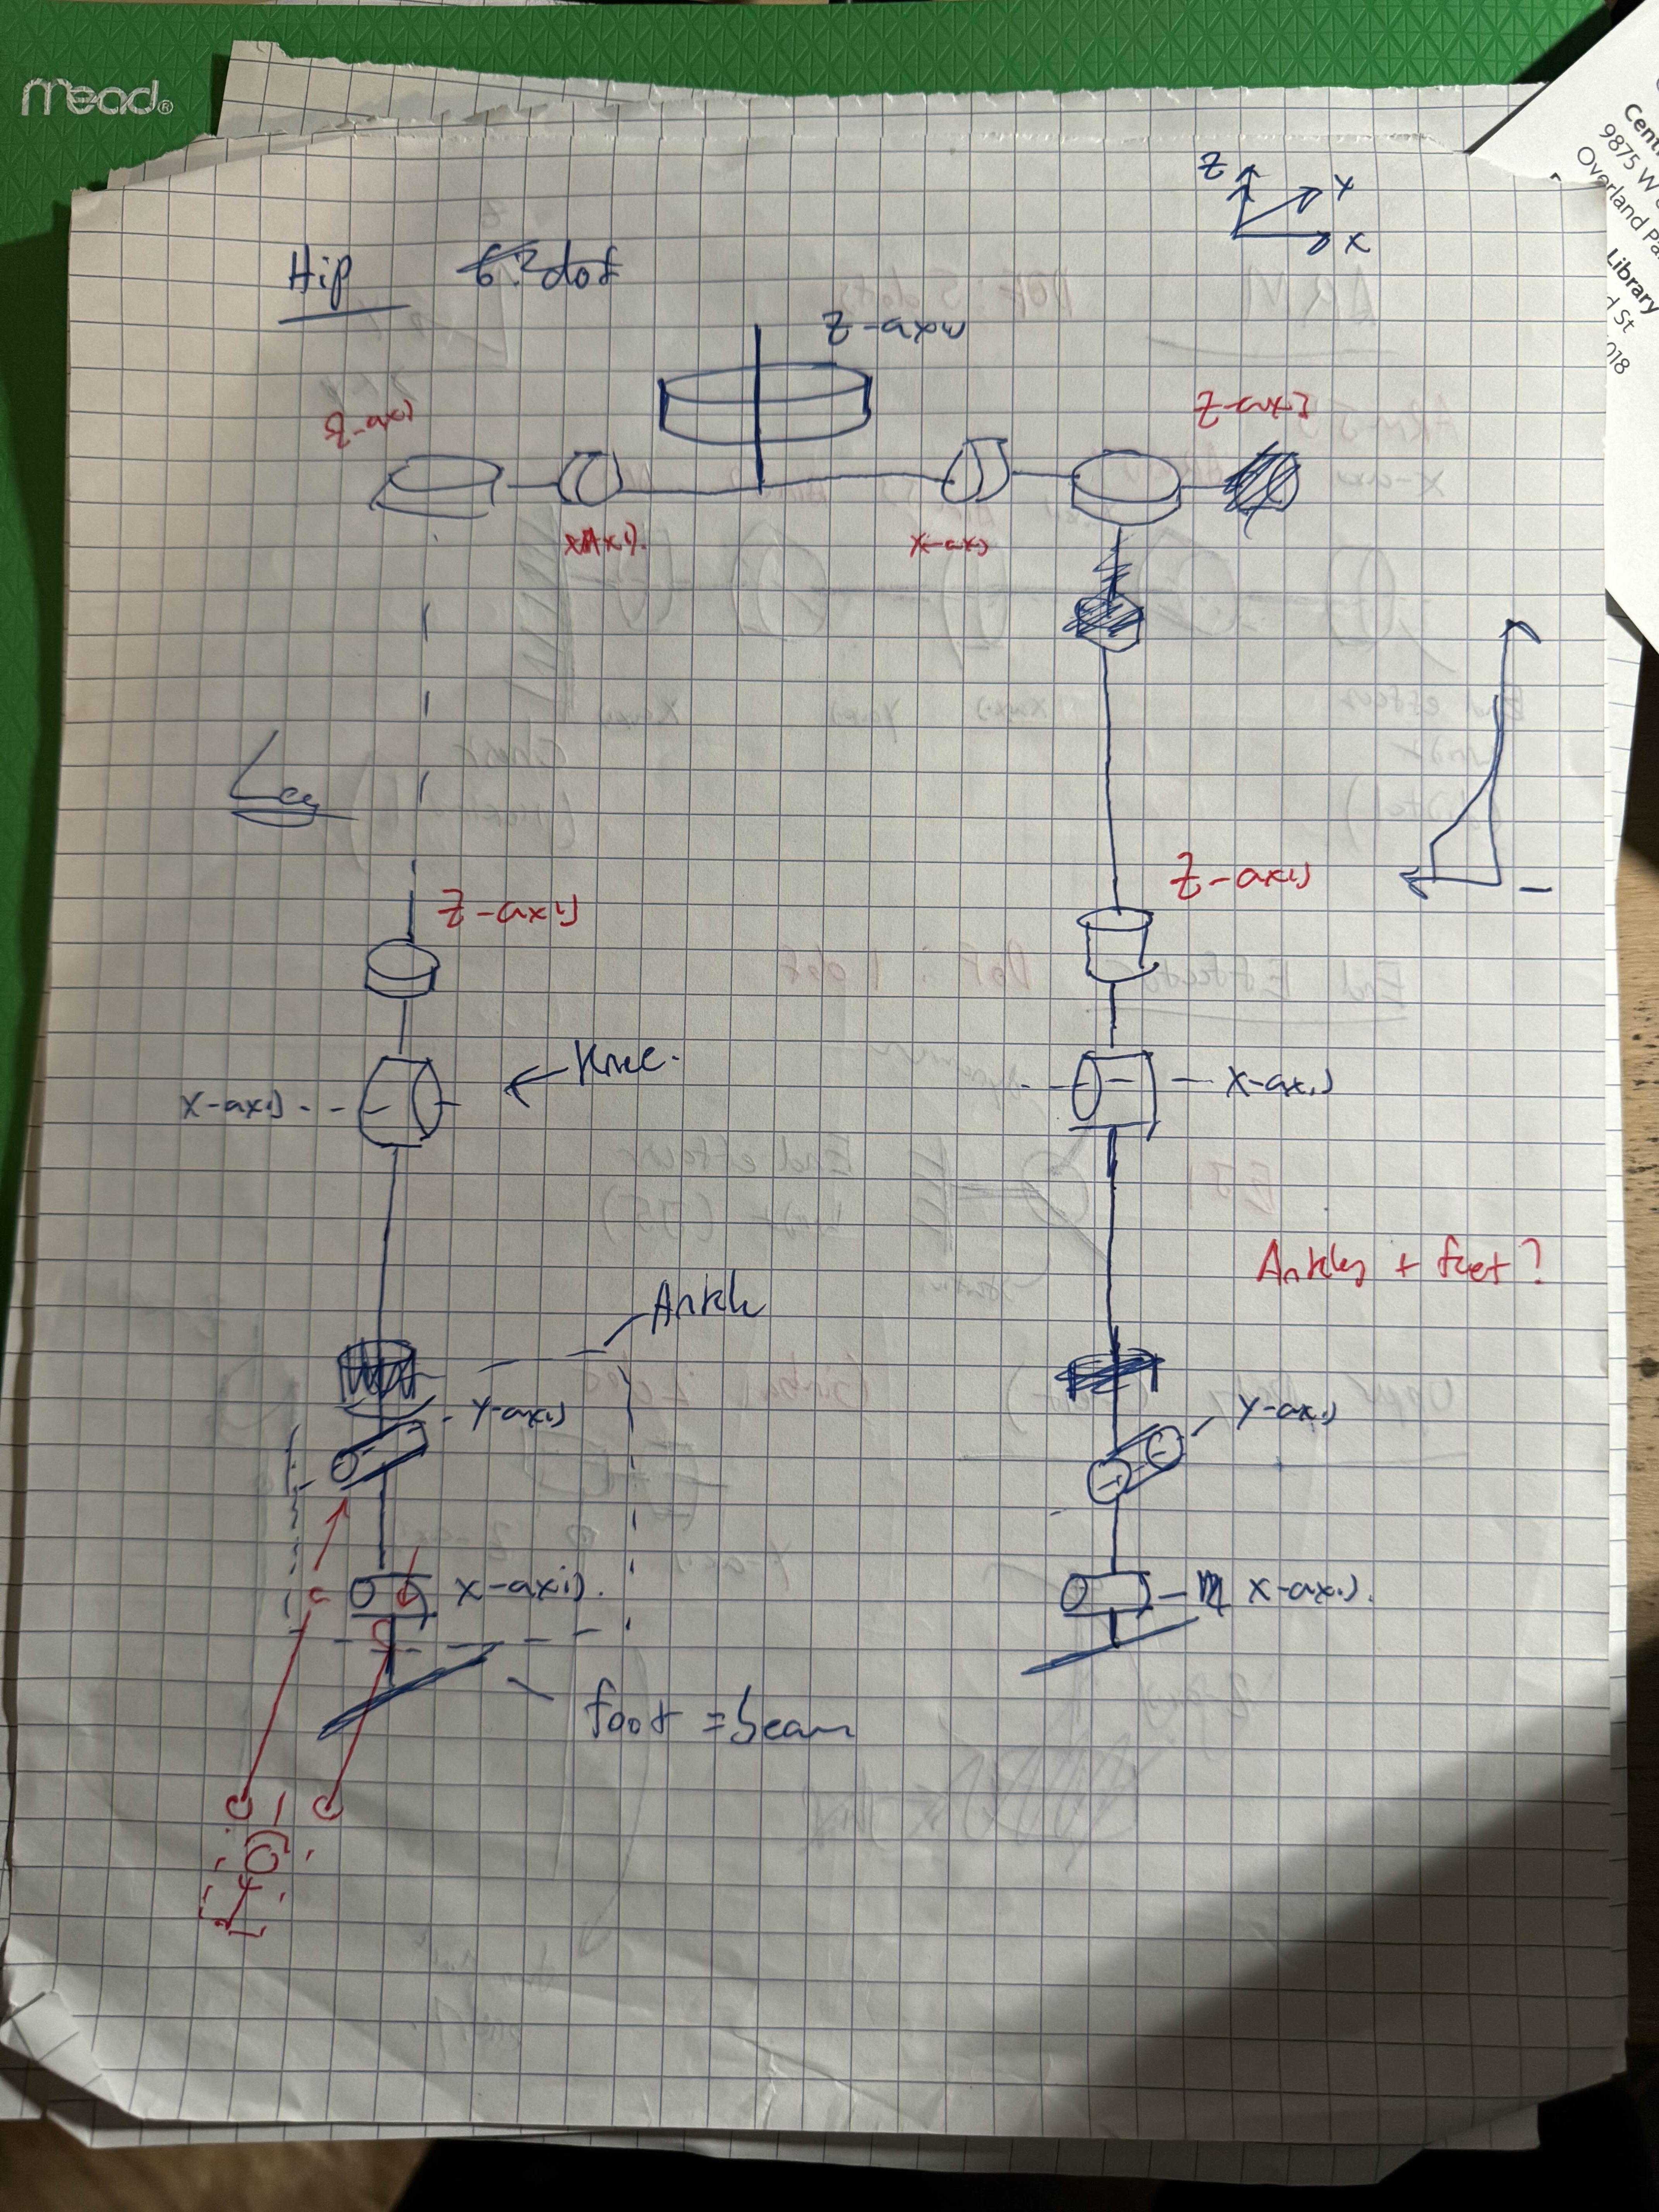
\includegraphics[scale=0.1]{assets/Design Presentation/Leg design 1.jpg}
    \caption{Revision 1 Leg and Hip Layout for Joints and Linkages}
    \label{fig:enter-label}
\end{figure}

\begin{figure}[H]
    \centering
    \includegraphics[scale=0.1]{assets/Design Presentation/Hip Rev 3.jpg}
    \caption{Revision 2 Leg and Hip Layout for Joints and Linkages}
    \label{fig:enter-label}
\end{figure}

\begin{figure}[H]
    \centering
    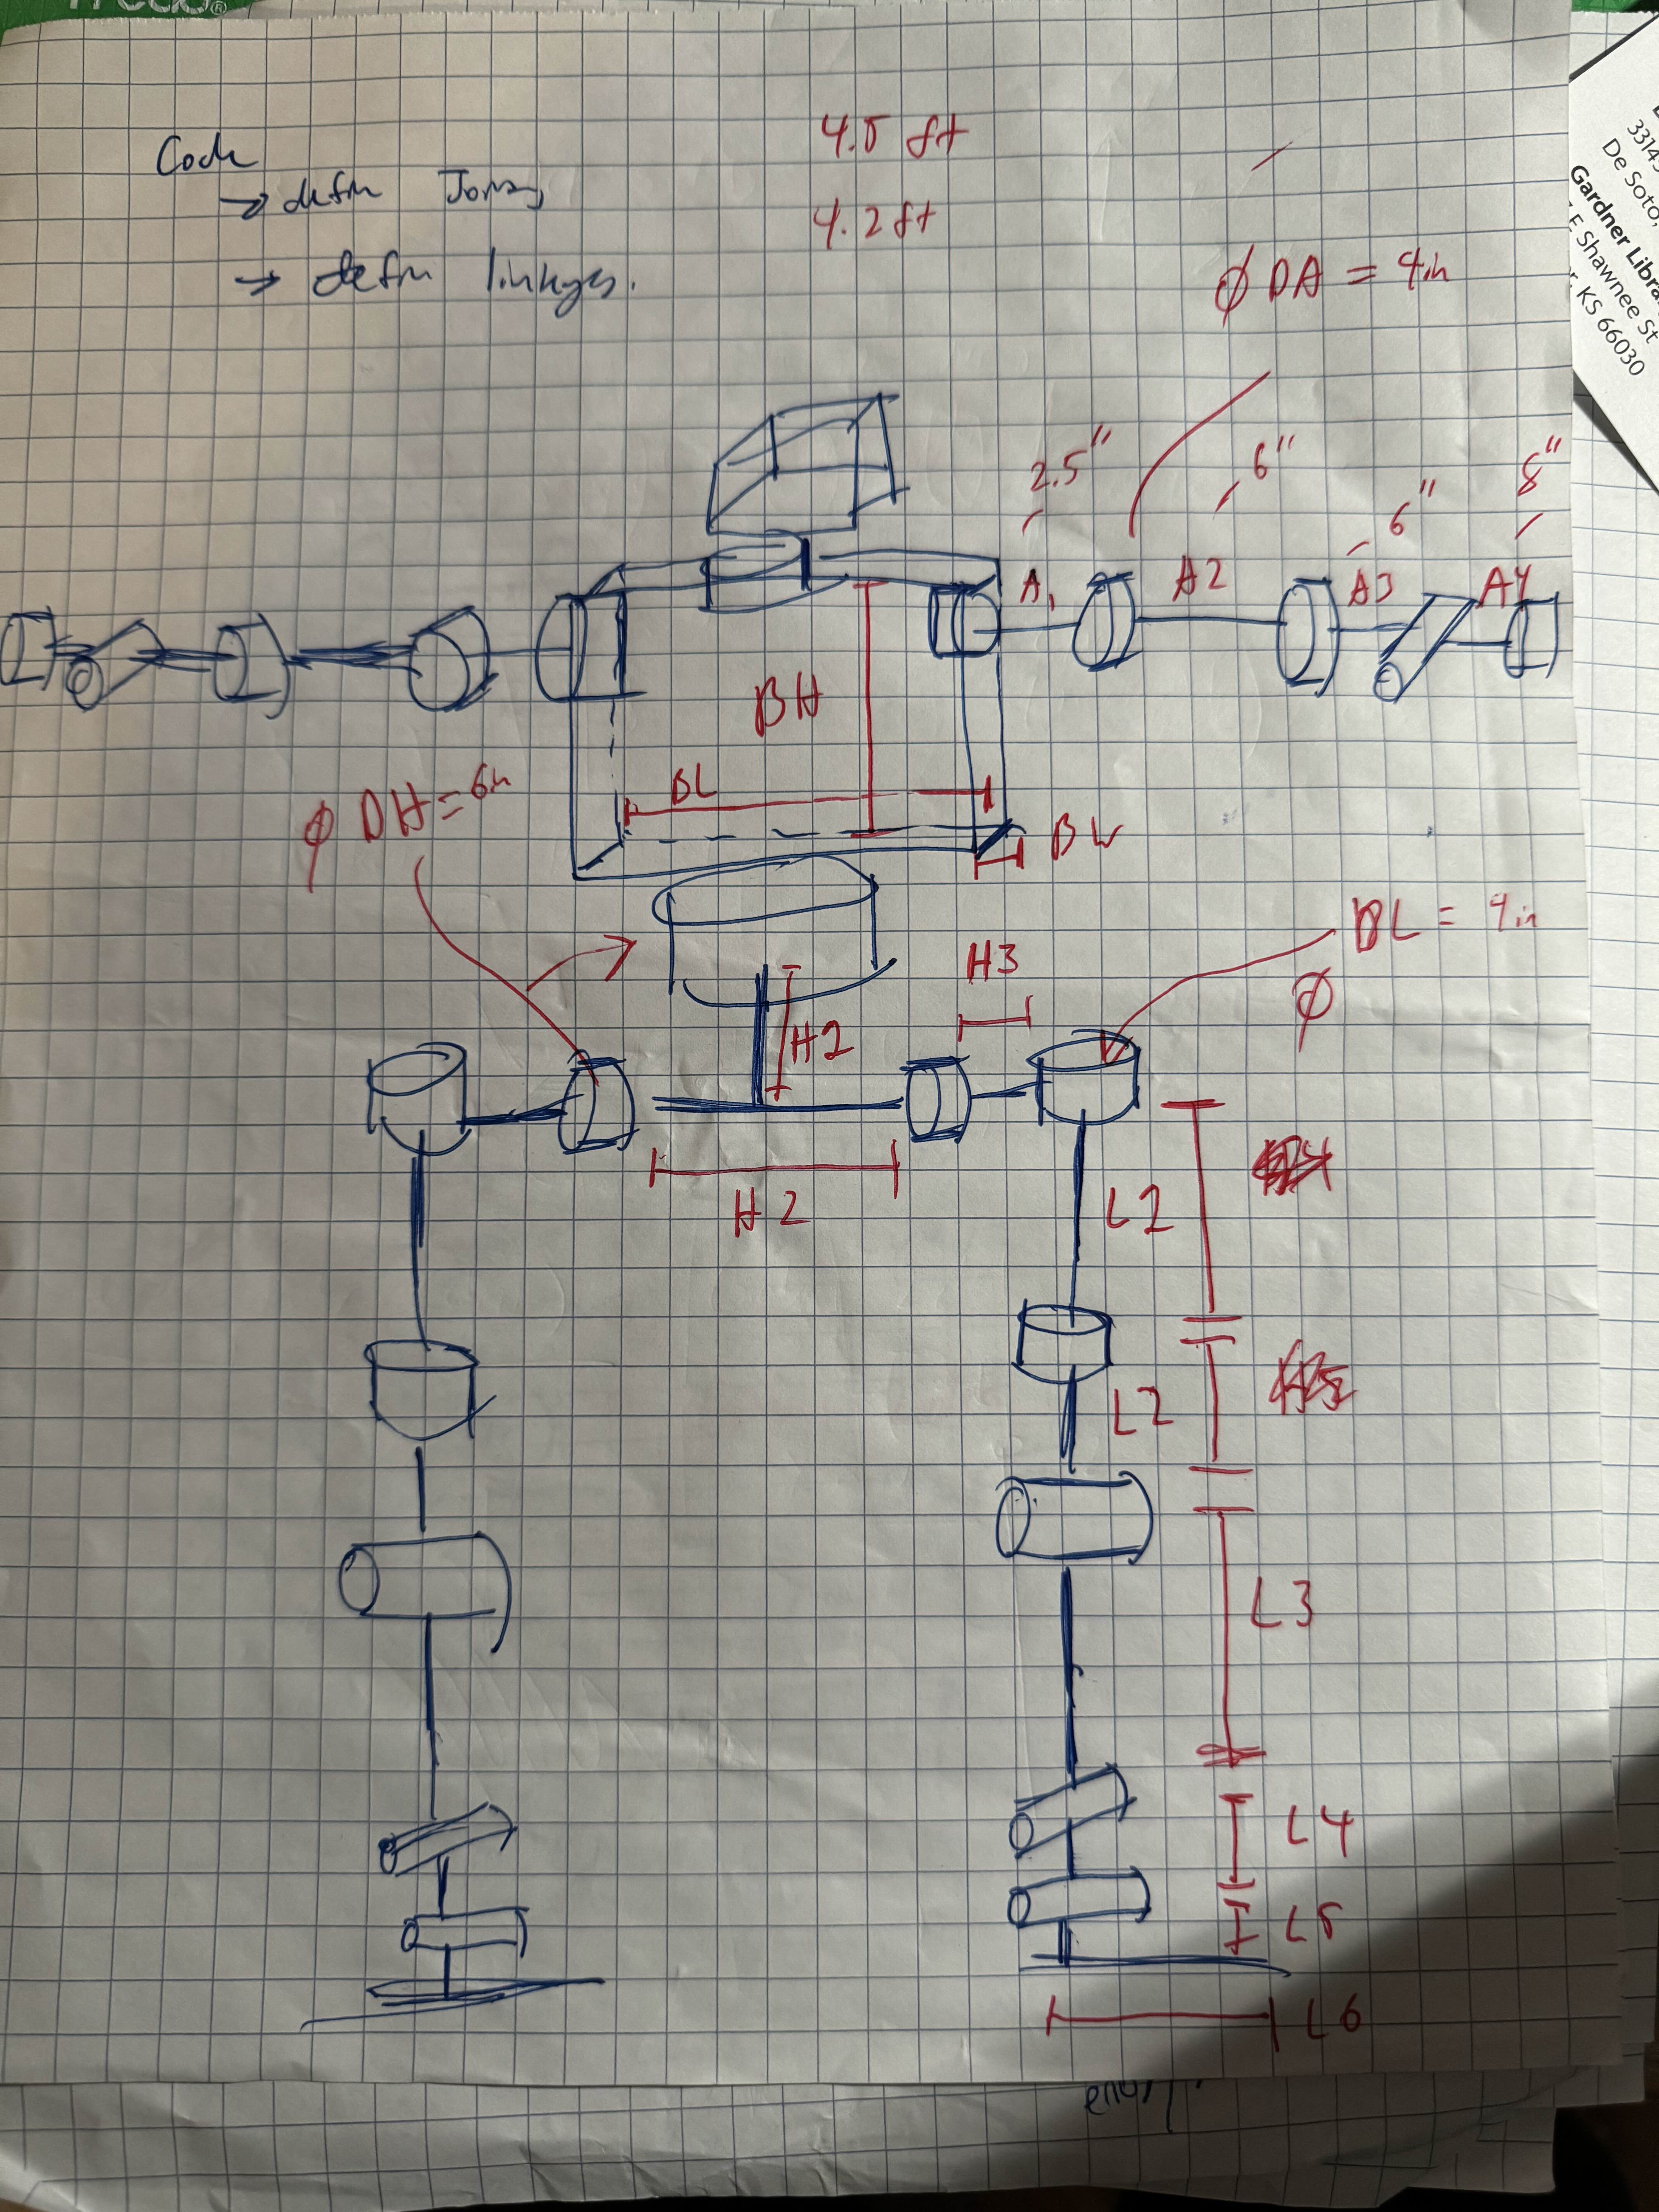
\includegraphics[scale=0.1]{assets/Design Presentation/MOHRA v1 layout.jpg}
    \caption{Revision 1 Full Humanoid Joint and Actuator Layout}
    \label{fig:enter-label}
\end{figure}

\begin{figure}[H]
    \centering
    \includegraphics[scale=0.1]{assets/Design Presentation/Layout Rev2.jpg}
    \caption{Revision 1 Full Humanoid Joint and Actuator Layout}
    \label{fig:enter-label}
\end{figure}

\newpage

\subsection{Moment Calculations}

\begin{figure}[H]
    \centering
    \includegraphics[scale=1]{assets/Design Presentation/Leg Layout Moments.png}
    \caption{Leg and Hip Layout \n Used for Moment Calculations}
    \label{fig:enter-label}
\end{figure}

\begin{table}[H]
\centering
\begin{tabular}{|>{\raggedright}m{4cm}|>{\centering}m{2cm}|>{\centering}m{2cm}|>{\raggedright\arraybackslash}m{6cm}|}
\hline
\textbf{Parameter} & \textbf{Qty} & \textbf{Units} & \textbf{Notes} \\ \hline
Mass: Link 5 and Link 4 & 0.7386 & Kilograms & \\ \hline
Length: Link 5 and Link 4 & 0.3294 & Meter & \\ \hline
Center of Mass Sum Link 4 and 5 & 0.1647 & Meter & Assume cylindrical tube with uniform geometry \\ \hline
Weight of Beam & 7.2459 & N & \\ \hline
Weight of Payload & 49.05 & N & Treated as point mass \\ \hline
Length: Joint 4 to Payload & 0.3294 & Meter & \\ \hline
Weight of Joint 5 & 8.6328 & N & Treated as point mass \\ \hline
Length: Joint 4 to Joint 5 (Link 4) & 0.2532 & Meter & \\ \hline
Moment: Beam (Link 4 and 5) & 1.1934 & Nm & Force * distance \\ \hline
Moment: Payload & 16.1571 & Nm & \\ \hline
Moment: Joint 5 & 2.1858 & Nm & \\ \hline
\textbf{Moment on Joint 4 (Sum of Moments)} & \textbf{19.5363} & \textbf{Nm} & \textbf{Rated Torque Spec} \\ \hline
\end{tabular}
\caption{Arm: Shoulder (Joint 4) Rated Torque Calculation}
\label{tab:joint4_torque}
\end{table}

\begin{figure}[H]
    \centering
    \includegraphics[scale=0.5]{assets/Design Presentation/Leg Torque Calcs.png}
    \caption{Leg Knee Joint Squat Torque Moment}
    \label{fig:enter-label}
\end{figure}

\newpage
\subsection{Actuators Considered}

\begin{figure}[H]
    \centering
    \includegraphics[scale=0.5]{assets/Design Presentation/Actuators_arm.png}
    \caption{Arm Actuators Considered Based on Rated Torque Requirements}
    \label{fig:enter-label}
\end{figure}

\begin{table}[h!]
\centering
\renewcommand{\arraystretch}{1.2}
\setlength{\tabcolsep}{10pt} % Adjust padding
\begin{tabular}{|l|}
\hline
\textbf{Supplier Name} \\
\hline
Anydrive \\
HEBI \\
ZeroErr (Faradyi) \\
MyActuator \\
CubeMars \\
MjBots \\
Dynamixel \\
LinEngineering \\
High Torque \\
Robstride \\
\hline
\end{tabular}
\caption{Actuator Suppliers Considered}
\end{table}



\newpage
\subsection{Required Rated Torques and Selected Actuators}
\begin{figure}[H]
    \centering
    \includegraphics[scale=0.5]{assets/Design Presentation/Arm Rated Torque and Specs.png}
    \caption{Arm Actuators Specified for MOHRA}
    \label{fig:enter-label}
\end{figure}

\begin{figure}[H]
    \centering
    \includegraphics[scale=0.5]{assets/Design Presentation/Leg Rated Torque and Specs.png}
    \caption{Leg and Hip Actuators Specified for MOHRA}
    \label{fig:enter-label}
\end{figure}

\newpage
\subsection{Actuator Costs}
\begin{figure}[H]
    \centering
    \includegraphics[scale=0.5]{assets/Design Presentation/Actuator Cost.png}
    \caption{Total Actuator Cost MOHRA}
    \label{fig:enter-label}
\end{figure}



\subsection{Skeleton CAD, KOL Image, and PPO ISAAC Image}
\begin{figure}[H]
    \centering
    \includegraphics[scale=0.5]{assets/Design Presentation/Skeleton Draft.png}
    \caption{Skeleton Model Layout}
    \label{fig:enter-label}
\end{figure}

\begin{figure}[H]
    \centering
    \includegraphics[scale=0.5]{assets/Design Presentation/KOL Build Skele.png}
    \caption{Skeleton Model Compiled in URDF Format}
    \label{fig:enter-label}
\end{figure}

\begin{figure}[H]
    \centering
    \includegraphics[scale=0.5]{assets/Design Presentation/Skele_ISAAC.png}
    \caption{Skeleton Model Loaded into ISAAC Gym}
    \label{fig:enter-label}
\end{figure}

\begin{figure}[H]
    \centering
    \includegraphics[scale=0.5]{assets/Design Presentation/Ministompy walking.png}
    \caption{Reinforcement Learning Model Training Mini Stompy to Walk}
    \label{fig:enter-label}
\end{figure}



\newpage
\subsection{MOHRA Top Level Assembly}

\begin{figure}[H]
    \centering
    \includegraphics[scale=0.15]{assets/MOHRA/MOHRA_Tpose.png}
    \caption{Complete Hardware Design for MOHRA}
    \label{fig:enter-label}
\end{figure}

\begin{figure}[H]
    \centering
    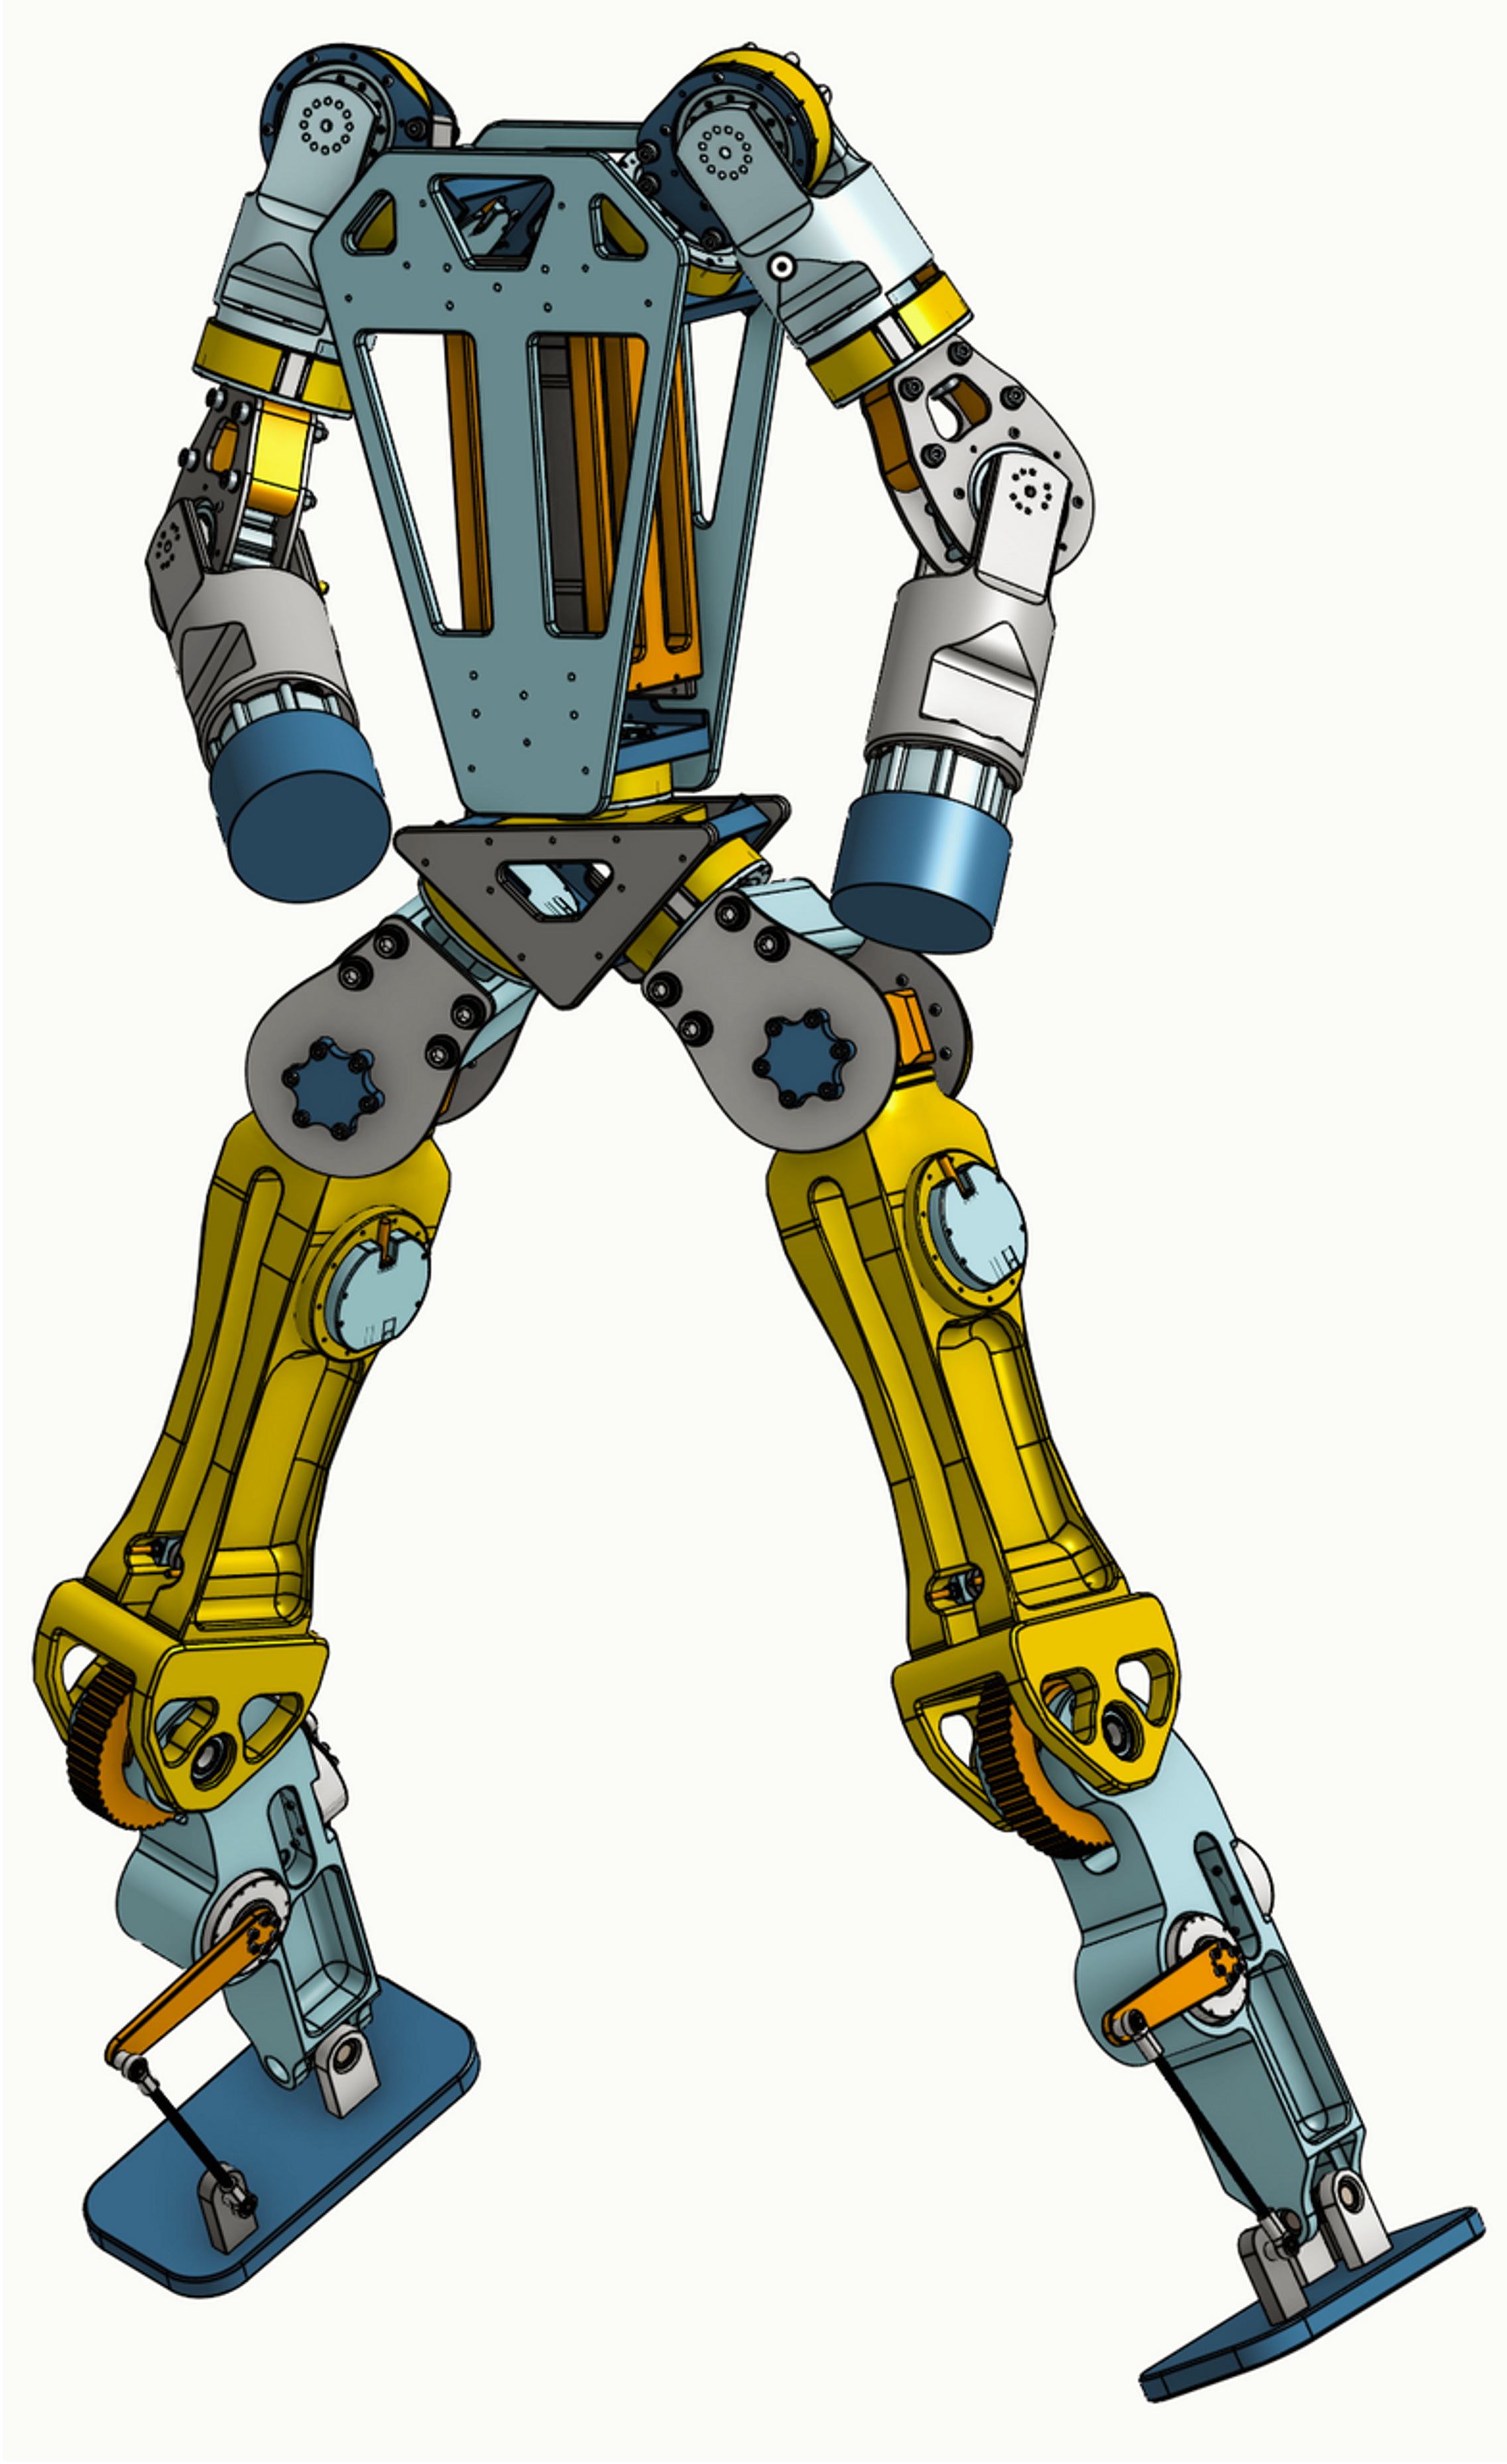
\includegraphics[scale=0.6]{assets/Design Presentation/MOHRA_v0.png}
    \caption{Front View MOHRA}
    \label{fig:enter-label}
\end{figure}

\begin{figure}[H]
    \centering
    \includegraphics[scale=0.6]{assets/Design Presentation/Back_MOHRA.png}
    \caption{Back View MOHRA}
    \label{fig:enter-label}
\end{figure}



\newpage
\subsection{MOHRA Sub-assembly Design: Arm, Trunk, and Leg}

\begin{figure}[H]
    \centering
    \includegraphics[scale=0.5]{assets/Design Presentation/MOHRA_Arm.png}
    \caption{MOHRA Arm Subassembly}
    \label{fig:enter-label}
\end{figure}

\begin{figure}[H]
    \centering
    \includegraphics[scale=0.4]{assets/Design Presentation/MOHRA_arm_section.png}
    \caption{MOHRA Arm Subassembly Section View}
    \label{fig:enter-label}
\end{figure}

\begin{figure}[H]
    \centering
    \includegraphics[scale=0.6]{assets/Design Presentation/MOHRA_Arm_housing.png}
    \caption{MOHRA Arm Actuator Housing}
    \label{fig:enter-label}
\end{figure}

\begin{figure}[H]
    \centering
    \includegraphics[scale=1]{assets/Design Presentation/Trunk Front View.png}
    \caption{MOHRA Trunk Subassembly Front View}
    \label{fig:enter-label}
\end{figure}

\begin{figure}[H]
    \centering
    \includegraphics[scale=1]{assets/Design Presentation/Trunk Rear View.png}
    \caption{MOHRA Trunk Subassembly Rear View}
    \label{fig:enter-label}
\end{figure}

\begin{figure}[H]
    \centering
    \includegraphics[scale=0.9]{assets/Design Presentation/Trunk Section View.png}
    \caption{MOHRA Trunk Subassembly Side Section View}
    \label{fig:enter-label}
\end{figure}

\begin{figure}[H]
    \centering
    \includegraphics[scale=0.8]{assets/Design Presentation/Leg Front View.png}
    \caption{MOHRA Trunk Subassembly Front View}
    \label{fig:enter-label}
\end{figure}

\begin{figure}[H]
    \centering
    \includegraphics[scale=0.8]{assets/Design Presentation/Leg Rear View.png}
    \caption{MOHRA Trunk Subassembly Rear View}
    \label{fig:enter-label}
\end{figure}

\begin{figure}[H]
    \centering
    \includegraphics[scale=0.8]{assets/Design Presentation/Leg Side View.png}
    \caption{MOHRA Trunk Subassembly Side View}
    \label{fig:enter-label}
\end{figure}

\begin{figure}[H]
    \centering
    \includegraphics[scale=0.8]{assets/Design Presentation/Leg Section View.png}
    \caption{MOHRA Trunk Subassembly Section View}
    \label{fig:enter-label}
\end{figure}



\newpage
\subsection{Mechanisms \& Transmissions}

%  images: belts, belt torque calcs, 4 bar linkage, ratios, linkage gif
\begin{figure}[H]
    \centering
    \includegraphics[scale=0.8]{assets/Design Presentation/Belt Drive.png}
    \caption{Belt Drive Mechanism}
    \label{fig:enter-label}
\end{figure}

\begin{figure}[H]
    \centering
    \includegraphics[scale=0.8]{assets/Design Presentation/Belt Drive Knee Output.png}
    \caption{Belt Drive Torque Output}
    \label{fig:enter-label}
\end{figure}

\begin{figure}[H]
    \centering
    \includegraphics[scale=1]{assets/Design Presentation/U Joint.png}
    \caption{Ankle Universal Joint}
    \label{fig:enter-label}
\end{figure}

\begin{figure}[H]
    \centering
    \includegraphics[scale=0.8]{assets/Design Presentation/Roll Linkage.png}
    \caption{4-Bar Linkage Roll Axis Ankle}
    \label{fig:enter-label}
\end{figure}

\begin{figure}[H]
    \centering
    \includegraphics[scale=0.8]{assets/Design Presentation/Torque Ratio Roll.png}
    \caption{Torque Ratio vs Roll Position Plot}
    \label{fig:enter-label}
\end{figure}

\begin{figure}[H]
    \centering
    \includegraphics[scale=0.8]{assets/Design Presentation/Roll_viz.jpg}
    \caption{Roll Linkage Visualization}
    \label{fig:enter-label}
\end{figure}

\begin{figure}[H]
    \centering
    \includegraphics[scale=0.8]{assets/Design Presentation/Pitch Linkage.png}
    \caption{4-Bar Linkage Pitch Axis Ankle}
    \label{fig:enter-label}
\end{figure}

\begin{figure}[H]
    \centering
    \includegraphics[scale=0.8]{assets/Design Presentation/Torque Ratio Pitch.png}
    \caption{Torque Ratio vs Pitch Position Plot}
    \label{fig:enter-label}
\end{figure}

\begin{figure}[H]
    \centering
    \includegraphics[scale=0.8]{assets/Design Presentation/Pitch_viz.jpg}
    \caption{Pitch Linkage Visualization}
    \label{fig:enter-label}
\end{figure}

\newpage
\section{Discussion}
\subsection{Overview}
The primary goal of this project has been to develop a robust general-applications robot design for the open-source ecosystem. Our final product is a fully designed and mated CAD assembly, with justification and documentation of most major tradeoff decisions and engineering calculations. The humanoid robot has 23 degrees of freedom: 5 degrees in each arm (roll-pitch-roll-pitch-roll), with the end effector left for future development; 1 degree of freedom in the waist; and 6 degrees of freedom in the leg, 3 at the hip (roll-pitch-yaw), 1 in the knee, and 2 (pitch-roll) at the foot. It is comprised almost fully of 6061-T6 aluminum, The final weight per the solid-body model is approximately 94.4kg (208lbs), with a height of approximately 1.66m and a wingspan of 1.66m. 

The estimated cost of the actuators came to approximately \$5,800. The other purchased components (fasteners, pulleys, etc.) amounted to about \$800 as well, with the current BoM predicting a cost of \$6650 (see \textit{Appendix F} for the itemized list). Due to delays and time limitations, we were unable to derive a specific cost for the aluminum stock and machined components, though it is expected that the final value will put our total cost of the assembly over the intended \$10,000 assuming that all manufacturing is outsourced. We do not believe that the stock itself will exceed the \$3000 mark; in the case that the user has the capability to perform the machining in-house, the \$10,000 may still be achievable. Further, as the actuators are imported products, the cost of this design may decrease significantly depending on the country.

\subsection{Limitations}
During the development of this robot, through our discussions and interpretations of the overarching need for accessibility for the open-source community, the most persistent constraint that arose was in making components simple to manufacture/acquire. This limited designs to profiles that can be made in a simple 3 or 3+1 axis mill/lathe within typical workspace sizes. This often drove the tradeoff of some additional weight and overall assembly complexity, as best showcased in the 3-part design of the upper leg; in terms of keeping stock sizes reasonable, having features reachable by standard tooling and making re-fixtures as few as possible, it proved to be a necessity (reference \textit{Appendix B: Legs, Thigh}), though it is likely to have added weight overall in terms of interfacing material and bolts. The bolt-together pinned joint yokes and the plates used for the main body structure follow a similar line of thinking, utilizing cheap 2-D cut parts (waterjet, lasercut, etc.) and fasteners for parts that would otherwise require complicated 3-D internal geometry or excessively large workspace sizes. 

In terms of conducting validation and analysis on the dynamic performance of our model, we specifically limited ourselves to the existing tools developed and published by K-Scale Labs. This was seen as essential to the point of having reproducible and accessible results -- favoring the open-sourced and established option, rather than trying to develop our own bespoke solution with limited outside reach and prospects for ongoing support. Further, it was an opportunity to assist K-Scale in proving out their own packages, our team being one of the first-comers in applying the tools outside of the K-Scale internal team. As we moved along in the project, this decision became a limitation in our progress. We came across many issues with bugs and dependency conflicts, and navigating these developing codebases proved rather difficult for the team. Understanding the process for implementing our models into the workflow and resolving the subsequent errors has been much more of a time and effort drain than initially expected. Some particularly inscrutable issues have delayed physics simulation and PPO training to beyond our timeline for the project. The K-Scale team working on flushing out documentation and instructions for use, and has been accessible and helpful to us in resolving various problems, so these issues will likely be resolved for future work; however, it has forced our team to scale back our expectations for this semester's work.

A knock-on effect of the simulation delays is in our light-weighting. Our first-pass assumptions for the mass/moment calculations proved to be rather severe under-estimates for the final weight of the components when motor interfaces, machining limitations, and transmission elements were incorporated; this in turn drove a push midway through design to trim away and shell large amounts of material. The extent to which we light-weighted our components was informed by reviewing the equivalent components on existing humanoid designs; however, proving the strength of our designs and identifying stress concentrations or unnecessary material relies on finite element models (static or topological optimization simulations), which themselves require relatively accurate data on the location, direction, and magnitude of dynamic loads. Without data from the simulation environments, we were therefore limited in the extent to which we could justifiably lightweight our components.  

As a final note on the limitations of our project, we would like to acknowledge the uncertainty on the performance and feasibility of our designs that comes with relying on a 3D CAD modeling and computer simulation. Though we were attentive to the accessibility of assembly features (e.g. fasteners) and the restrictions to feature geometry that come with 3-axis machining, it is likely that there are some oversights in unnecessarily hard-to-machine profiles, unsuitable fixturing features, hard-to-service components, and other annoyances that will only be caught when programming the machining toolpaths and fastening the physical parts together. Further, without running the robot in the real world, the performance impacts of the many effects neglected in our analyses -- joint friction and stiffness, deflection and misalignment of structural elements, unexpected load conditions -- will not be understood. Recording motor diagnostics, employing strain gages on concerning features, and stress-testing the mobility of the robot in various terrains is all necessary to validate and further iterate this design. Though the cost and time commitment to doing this sort of analysis proved well outside of the reasonable scope of this project, it is the necessary next step once the current simulation issues are resolved and we (or future users of the open-source model) are able to confidently lightweight excess material throughout MOHRA.

\subsection{Final Design}
All of this said, we have gained some key insights into humanoid design throughout the process of creating this humanoid model. More extensive and specific discussion to this effect is done in \textit{Appendix B}; we will discuss the higher-level takeaways here.

Although the legs were determined to be the larger focus for our design, there are many advantages to beginning the design process with the arms. Support of the mass of the arms and the loads carried through them is flowed through the rest of the robot, informing the designs of the trunk and the legs. Proving out an accurate expectation for the arm dimensions and mass early on therefore reduces the need to revise the other sub-assemblies. It is almost assured that any initial length choices for the arm links will need to be adjusted when getting to the prototype design phase. Our team had particular trouble in achieving as short a distance from the shoulder roll to pitch joint as intended; ideally they would be coincident, in terms of limiting inertial effects, but we determined the offset distance had to be increased after establishing how much space was necessary to transition a longitudinal motor interface into a transverse mount. Due to the lack of clear load cases that comes with designing a general purpose robot -- the arm end effectors may be applied towards any number of specific applications -- we  expect that the strength, and therefore the weight, of the arm structure will need updated for each implementation. That said, though we believe that our design will act as a reasonable baseline once the aforementioned simulation and lightweighting is performed.

Concerning the main body of MOHRA -- the trunk, waist, and initial hip 'yaw' joints -- this is the most pressing area for cost reduction, as it forms the largest continuous pieces of material in the humanoid. It is important that the various mounting locations throughout the body be accurately and rigidly connected, so we chose to have the mounting locations all be machined in a single operation, of a single piece of stock. To accommodate this, we specifically chose to utilize large 2-D cut plates for locating and providing the main structural support between all of the motor mounts and the battery pack. The same design approach was carried into the hip design, using the same parts in service of reducing overall complexity and cost. Further, we chose to re-use the removable battery pack from the existing mini-stompy design for interoperability and simplicity -- again sacrificing some theoretical mass efficiency for ease of sourcing and implementation. 

Looking to the legs, these proved the most complicated and difficult components in an engineering and design sense. Given they simultaneously see the most load overall and have the most degrees of freedom (neglecting any end-effector in the arm), designing the legs was an ongoing struggle of keeping elements structurally sound and still fitting all of the mounting/interfacing points for the motors and transmission elements. In service of decreased moment of inertia overall, there is incentive to have all motors move as close to the trunk as possible, naturally pushing them all to be effectively on top of one another. We were able to do this, especially in the hip design, but the adjacent mounts and structural links had to be made larger -- that is, heavier and generally weaker under moment loads -- as a result. We learned through this process that adding degrees of freedom cannot simply be evaluated as incurring the weight of the motor and any corresponding transmission parts; there is also a major factor in the material needed to mount and deflect the main structural load-paths around these elements. Keeping things easily machinable was also a concern. Due to the interfacing issue -- having so many mounting points fighting over space -- and how it interacted with the lightweighting process and our machining limitations, we chose to split the upper leg over multiple pieces. Further, with the main body of this upper leg as well as the lower leg requiring features on almost all sides, the apparent machining complexity ballooned in terms of re-fixtures and, accordingly, the difficulty of keeping all features correlated.

\subsection{Overarching Takeaways}

Considering MOHRA, in its development, current design, and future, our team has a few key design beliefs that we feel will be vital to continue forward with. 

Firstly, an attention to safety is as vital as in any other application. Though there is much left to do to bring MOHRA into reality, we have given some early attention to reducing opportunities for pinch-points (packaging the belt interior to the leg) and limiting the possibility of the robot to damage the environment/people around it (backdrivability in the motors is useful in this regard). As the prototype model is further refined, continued efforts in guarding, lightweighting, and mechanical/electrical stops will be essential for conscionable proliferation of this design. 

Secondly, continued cooperation with K-Scale in the software simulation and control system development process will remain an important aspect of the project scope. Though we ran into many issues with successfully implementing these early versions of the import-and-simulation workflows, the underlying structure and intention of the software ecosystem that K-Scale is developing nonetheless is an essential aspect of the MOHRA project. Fully oriented towards lowering the barrier to entry in accessing humanoid designs and accelerating users' engagement with the subject, this ecosystem will serve to benefit the reach of the MOHRA design, and our ongoing communication with the K-Scale team has assured us that it will continue to be supported into the future.

Finally, the choices to keep manufacturing methods and component selection accessible should be seen as an advantage to the future success of this prototype model. As we have elaborated upon, there have been many tradeoffs in specific performance and capability that came due to our imposed limitations. However, given how volatile, uncertain, and rapidly innovating the humanoid space is currently, we see that optimizing our design to the exclusion of all else is the incorrect pathway to follow. The advantage to the open-source nature of this design is that it allows more intelligent and engaged designers to contribute to moving humanoid robots forward as a field of study and market. In this, there is a need to develop a performant design -- to attract interest in its own right -- but never to the exclusion of getting it in people's hands.

\section{Summary and Conclusions}
%recap of project and outcomes, discuss why and why we did not meet deliverables

The machined open-source humanoid robot architecture (MOHRA) project set out to design a humanoid robot that made of machined Aluminum components and off the shelf actuators. We focused on making our design accessible to the open-source community by reducing costs of machined hardware and actuators where possible and increase the simplicity in the assembly of our hardware. The mechanisms and actuators we selected and designed were chosen based off of static moment calculations and appropriate mechanism calculations to validate our design choices documented in Appendix B. We also set goals to validate our design using K-Scales software simulation tools in order to train our designed humanoid to stand and walk in an ISAAC gym simulation environment. The result of our work was a 23 degree of freedom humanoid robot that utilized Robstride planetary gear actuators. Our humanoid weighed a total of 94.42kg and was made of machined 6061 Aluminum. Our design choices for the machined components came down to reducing the mass where possible, ensuring there was defined mounting points for actuators, and defining the clearances for mechanism operation and envisioned cable routing. We specified actuators based on the maximum static moment load case that the joint was expected to sustain loads on and made extra considerations around the load case of the knee joint. The knee and ankle joints were designed to ensure that we maintained desired torque output while minimizing the increase in moments during limb actuation. We selected the belt drive and 4 bar linkage for the knee and ankle joints respectively due to their lower complexity in design and assembly and lower costs to stay aligned with our mission of ensuring our design could be utilized by the open-source community. We created a complete CAD model of our hardware design that is publicly accessible in OnShape and for individuals to use for hardware or software purposes. We made significant effort to validate our designed hardware using the software simulation tools created by K-Scale, but we did not successfully get our OnShape models to train to stand or walk due to software issues. We relied on the software simulation to give us physical load data on our joints and due to the inability to get software simulation to work we were unable to gather load data on our hardware that could be used for additional light weighting. Despite this, we invested significant effort into utilizing Ntopology to explore potential solutions to light weight components to further improve our design. We met the deliverable of designing and defining a CAD assembly for a machined humanoid but we were unable to validate it in simulation due to some training issues. We believe that despite the inability to get the simulation functions working by testing the software tools created by K-Scale we have helped to improve the code and the documentation for them for future use cases resulting in improving the software functionality. We created a bill of materials for our hardware design and required off the shelf components. To further investigate final costs of MOHRA communicating and negotiating with machine shops will be necessary to understand the costs of the machined components. What we have created is now a starting point those that are interested in Humanoids can reference for their own project or iterations to further accelerate the rate of development and raise the number of individuals involved in humanoid robot design.
%suggest possible improvements and next steps
In pursuit of improving our initial design there is a few aspects that can be investigated. The MOHRA design currently stands at 94.42kg which is quite heavy relative to other humanoids on the market today. There is significant room for reducing the weight of our hardware which may also in turn reduce the costs for the hardware required. In addition, transitioning some of the hardware from Aluminum to composite plastics or other materials that can sustain the loads would be favorable to mass efficiency gains. The simulation validation work can be further pursued to debug and resolve the issues associated with training our hardware design in ISAAC gym. Further collaboration with K-Scale and in depth development can be pursued to enable the hardware we have designed to be trained to walk or stand and enable the collection of load data for further FEA analysis for design validation. Completing software validation work can also be used to deliver further insights into joint functionality and overall joint layout optimization to improve the humanoids capability to walk or perform various actions. In addition, training the platform to perform additional actions is also an avenue towards understanding the limitations and abilities of our design. Finally, developing the embedded electronics and creating a concrete electronic system layout plan based on K-scales electronics and software platform would be the next steps to defining the necessary components required for fabrication, assembly, and testing.  




\newpage
\addcontentsline{toc}{section}{References}
\bibliographystyle{IEEEtran}
\bibliography{refs}


\newpage
\section{Appendix A: Team \& Project Organization}

\newpage
\subsection{Gantt Chart}
\includegraphics[scale=0.2, angle=90]{assets/ProjectManagement/emae_398__mohra_2024-12-06_11.53pm.png}

\subsection{Budget}
\begin{table}[H]
\centering
\begin{tabular}{|>{\raggedright}m{3cm}|>{\raggedright}m{2cm}|>{\centering\arraybackslash}m{1cm}|>{\raggedright}m{4cm}|>{\raggedright\arraybackslash}m{5cm}|}
\hline
\textbf{Budget Item} & \textbf{Cost} & \textbf{Qty} & \textbf{Product Type} & \textbf{Notes} \\ \hline
OnShape & \$0.00 & 2 & CAD Software & Student License \\ \hline
nTopology & \$0.00 & 1 & Optimization Software & Student License \\ \hline
Nvidia ISAAC Gym & \$0.00 & 2 & Simulation Software & Open Access \\ \hline
Overleaf & \$0.00 & 2 & Word Compiler & Free Service \\ \hline
Github & \$0.00 & 2 & Version Control Software & Free Service \\ \hline
Python & \$0.00 & 2 & Programming Language & Open Access \\ \hline
Google Suite & \$0.00 & 2 & Software Suite & Free Service \\ \hline
\multicolumn{2}{|r|}{\textbf{Total Cost:}} & \multicolumn{3}{l|}{\textbf{\$0.00}} \\ \hline
\end{tabular}
\caption{Budget Table}
\label{tab:budget}
\end{table}

\subsection{Project Advisor Meeting Log}

\begin{longtable}{|>{\raggedright}m{2.5cm}|>{\raggedright}m{2.5cm}|>{\raggedright}m{4cm}|>{\raggedright\arraybackslash}m{6cm}|}
\hline
\textbf{Date} & \textbf{Meeting Time} & \textbf{Attendees} & \textbf{Notes} \\ \hline
\endfirsthead
\hline
\textbf{Date} & \textbf{Meeting Time} & \textbf{Attendees} & \textbf{Notes} \\ \hline
\endhead
8/27/2024 & 2:30-3:00 pm & Dr. Hostler, Joshua Huang & Initial scope discussion and schedule cadence. \\ \hline
9/5/2024 & 3:30-4:00 pm & Dr. Hostler, Ian Dyke, Joshua Huang & Next Steps: Project Charter, WBS, Open source considerations, preliminary research. \\ \hline
9/12/2024 & 3:30-4:00 pm & Dr. Hostler, Ian Dyke, Joshua Huang & Presented Gantt Chart, defined project status in the planning phase, technical reading work, and clarifications on the risk mitigation plan. Checking the final presentation date works for Dr. Hostler. \\ \hline
9/26/2024 & 3:30-4:00 pm & Dr. Hostler, Ian Dyke, Joshua Huang & Provided updates on CAD work, defined DOFs, plans for importing CAD to SIM, and chose to create CAD to determine torques. Details on meeting with Dr. Daltorio for design insight. \\ \hline
10/3/2024 & 3:30-4:00 pm & Dr. Hostler, Ian Dyke, Joshua Huang & Presented updates on CAD model, demo of working Onshape to URDF pipeline. Discussed design details and direction using pipeline in the overall workflow. Discussed next steps of exporting model to physics SIM. Transitioned to work on final report draft. \\ \hline
10/17/2024 & 3:30-4:00 pm & Dr. Hostler, Ian Dyke, Joshua Huang & Presented trained mini stompy demo walking in ISAAC Gym. Torque calculation progress for motor specs. General focus on upper body hardware design right now. Updates on work to define custom skeleton model for use in ISAAC gym. \\ \hline
10/24/2024 & 3:30-4:00 pm & Dr. Hostler, Ian Dyke, Joshua Huang & Presented updates on completed torque calculations for arms accounting for mass of links, payload, and actuators. Presented assessment of existing actuators and decision justification for Robstride motors. Shared updates for next steps focusing on CAD design and dimensions built from actuators spec’d. Provided updates on Skeleton.py scripting issues preventing deployment to ISAAC Gym. \\ \hline
10/31/2024 & 3:30-4:00 pm & Dr. Hostler, Ian Dyke & Provided updates on CAD progress and NTOP optimization for mesh design. \\ \hline
11/7/2024 & 3:30-4:00 pm & Dr. Hostler, Ian Dyke, Joshua Huang & Presented progress on arm and trunk CAD outline and definition. Creation of first integration of actuators into arm hardware. Lower leg torque calculation approach defined. \\ \hline
11/14/2024 & 3:30-4:00 pm & Dr. Hostler, Ian Dyke, Joshua Huang & Presented completed arm hardware CAD, preliminary leg configuration layout, and I-beam calculations for mass. Completed leg and knee-rated torque requirements based on calculations. \\ \hline
11/21/2024 & 3:30-4:00 pm & Dr. Hostler, Ian Dyke, Joshua Huang & Presented arm lightweight concerns, belt drive for knee actuator, trunk CAD, and progress updates on software design. Updates on design reviews based on discussions with K-Scale. \\ \hline
12/5/2024 & 3:30-4:00 pm & Dr. Hostler, Ian Dyke, Joshua Huang & Presented overall updates after final presentation and intersections poster submission. Discussed final report plan and walked through debrief of project. \\ \hline
\caption{Project Meeting Schedule and Notes}
\label{tab:meetings}
\end{longtable}

\subsection{Work Breakdown Structure and Task List}
\includepdf[page=-, angle=90]{assets/ProjectManagement/EMAE 398_ MOHRA WBS_Task List - Sheet1.pdf}
\newpage

\subsection{Risk Mitigation Plan}
\includepdf[page=-, angle=90]{assets/ProjectManagement/EMAE 398_ MOHRA Risk Mitigation Plan - Sheet1.pdf}
\newpage

\section{Appendix B: Subassembly In-Depth Design Description}

\subsection{Layout Decisions}

MOHRA's initial schematic was made with a basic foundation in the Mini-Stompy design from K-Scale. This is a basis of a 5-DoF arm (neglecting the wrist/hand) in a roll-pitch-roll-pitch-roll configuration, and a 5-DoF leg with a roll-yaw hip interface and a roll-pitch-pitch lower leg configuration. This matches the primary rotational modes of human limbs. 

Upon review of peer robots with attention to common joint layouts and the apparent performance improvements that came alongside additional Degrees of Freedom, additional joints were added to our design scheme:

 \begin{itemize}
     \item A central "waist" vertical roll degree of freedom was added to the trunk, to allow for upper body action separate from walking motions -- that is, not being stuck in "tank control" mode bound to the legs when reorienting the trunk and arms.

    \item An additional longitudinal (roll) degree of freedom was added to the ankle to permit more responsive walking dynamics. From analysis of peers
    \cite{pndboticsAdam} \cite{pndbotics_adam_vid_2024}
    this appears to provide significantly benefits to lateral walking movements and general capability in traversing more complex environments, as compared to only having a pitch up/down of the foot. 
 \end{itemize}

Later in development, the decision was made to align the initial shoulder and hip roll axes offset 45 degrees from the horizontal. This was inspired by the PNDBotics Adam robot. This allows the limb assemblies to be brought closer inwards, reducing some undesirable moments and inertial effects on the waist, and provides for a more human-like range of motion in the inverse kinematics. In addition, mounting the shoulder actuators in the trunk area rather than as independent to the trunk allows the concentration of additional mounting hardware and material required for mounting closer to the center of mass of the trunk of the humanoid rather than additional additional moments on the trunk due to the mounting hardware necessary to attach the shoulder actuators. 


\subsubsection{Actuator Placement}

% Move things up 

\subsubsection{Body Moment Calculations}

Moment calculations were performed in order to determine the maximum static moment load case on an actuator that it would be required to operate under. To do this the mass of each linkage and joint must be defined and for starting initially it is best to determine the approximate linkage geometry like tubing or I beam to begin with in order to make sure your approximations are close to the final design. The next thing to do is understand the position of each joint and this is dictated by the length of all the linkages. To determine the moment that each joint experiences you treat the joint of interest as a cantilevered beam with a pivot point fixed to the datum vertical wall. All the of linkages and actuators distal to the actuator torque load of interest are accounted for during the moment calculation. The linkage masses are summed together to determine the total mass that will be treated as a beam with assumed evenly distributed mass. The center of mass of the beam is then defined in order to determine the distance from the pivot point that the moment will be acting at. Next the weight of the actuators is determined and the distance away from the pivot points is defined in order to determine moment that it is actuating on the pivot point. The sum of all of the moments including the moment of the linkage and the moments from the actuators is accounted for in order to determine the max torque load due to the hardware. In the event that an added payload capacity is desired, a defined capacity weight is defined and the distance away from the pivot point is defined that can be added to the total moment on the pivot point. This static analysis defines the maximum rated torque load that an actuator should be capable of sustaining at the joint. This was done for both the legs and the arms of the humanoid joints. 
An additional consideration for the static loads that were larger than the cantilever load case was the squat of the humanoid joint. The bending angle of the knee joint, the mass of the upperbody, and how spread apart the feet were from the other feet are the key factors that determine the moment load. The angle and width that the feet are spread apart will define the length of the moment arm and ideally the moment arm is shorter to reduce the load. To achieve these lower loads limiting the knee bend and assuming a larger food to foot width will reduce the length of the moment arm. Finally, the weight of the upper body should be reduced in order to reduce the total moment on the knee joint from the upper body. 

Some other cases that we did not explore but could be explored are the static forces from various terrain or platforms that the foot is pushing of off but we assumed that our gait was not actuating forces in the tibia or ankle in order to return force to the hip. Typical human gaits use the normal force when walking to perform walking and moving forward rather than upward which is much more efficient. A large problem with modeling this is that it is a statically in-determinant load case during since there are more unknowns than knowns when trying to model the loads, degrees of freedom, and the unconstrained datum that would be desired for the approach of calculating the moment on the joint. This is where pulling in moment or load forces on the actuators from the ISAAC simulation could prove useful to further validate or evaluate joint loads to ensure that the system is functional and does not require additional torque. 

\subsubsection{General Machining Constraints}

In service to making this open-source design approachable for as many as possible, we planned the designs of all of our machined components around using a basic 3-axis CNC mill. As a representative for this, we chose the HAAS VF1 was chosen, with a workspace limit of 20x16x20" / 508x406x508mm XYZ \cite{haas_vf-1_nodate}. In general, we strove to reduce the number of individual faces needing to be machined on parts to reduce the necessary re-fixtures needed for manufacturing; however, cost and functionality concerns limited how well we could apply this principle in many instances. Where it was possible to reduce cost and eliminate particularly annoying geometry by splitting components into 2-D cut (waterjet, plasma) profiles to be bolted together, we favored doing so.

\subsubsection{Draft Model}

\begin{figure}
    \centering
    \includegraphics[width=0.75\linewidth]{assets//Skeleton/Skele_FlyingKick.png}
    \caption{Skeleton CAD Design}
    \label{fig:enter-label}
\end{figure}

The first development of MOHRA began with a draft 'Skeleton' model. This served two main purposes:

1 - A basis for visualizing our initial joint length estimates. We were unable to find any established methodology for selecting specific limb lengths nor the proportions of the individual links comprising the limbs, and as such the lengths were driven by typical human body proportions. As example, it is common that the upper arm is approximately the same size as the foot; for a 5.5-6 foot tall male, the foot is approximately a foot (unit), and as such the initial upper arm was chosen to be 11" total length. The visualization allowed for determining if any proportions felt qualitatively "off" relative to human proportions. These dimensions would later be modified to align with specific torque calculations and packaging/interfacing limitations.

As a component of this, the shoulder width was defined as a function of arm range of motion.
%%% CONTINUE THIS -- get a snip of the Range of Motion Study thing in MOHRA drive. I can't access rn for some reason ~ josh
\begin{figure}
    \centering
    \includegraphics[width=0.75\linewidth]{assets/Skeleton/Rangeofmotionstudy.png}
    \caption{Arm Range of Motion Study}
    \label{fig:enter-label}
\end{figure}


2 - An initial model for proving out the CAD-to-Sim workflows established by K-Scale. The limited part count and mate tree provided quicker troubleshooting and processing of the model through this system.

\subsection{Arms}

\begin{figure}
    \centering
    \includegraphics[width=0.75\linewidth]{assets//MOHRA/MOHRA_Arm.png}
    \caption{MOHRA Arm}
    \label{fig:enter-label}
\end{figure}

The development of MOHRA began with the Arms. For our general-purpose-performance intent, they were seen to have little dependence on the legs for their own functionality, whereas the trunk and lower body need approximate arm weights to define static requirements.  

The design of the arm was concluded at the 'wrist' axial roll joint; it is our understanding that end effectors are highly complicated and generally design with a specific end goal in mind, and as such they were deemed out-of-scope for our general-purpose humanoid.

\subsubsection{Arm Layout}

The initial arm lengths are defined as previously described. In the process of laying out the solid bodies for the arms, it was found that the spacing allotted for the upper arm joints was too short to allow for the actuators to be added in-line; rather than incur additional weight and complexity from offsetting the mount interfaces, the spacing was increased to accommodate the motors. This amounted to (6"+5"=) 11" growing to a (202.4mm + 127mm=) 329.4mm = 12.96" upper arm length.

\subsubsection{Pitch Joints}

\begin{figure}
    \centering
    \includegraphics[width=0.5\linewidth]{assets/MOHRA/Sub-Arm/ShoulderPitch_Front.png}
    \caption{Shoulder Pitch Actuator}
    \label{fig:enter-label}
\end{figure}

\begin{figure}
    \centering
    \includegraphics[width=0.5\linewidth]{assets/MOHRA/Sub-Arm/ShoulderPitch_Rear.png}
    \caption{Shoulder Pitch Actuator Housing}
    \label{fig:enter-label}
\end{figure}

The pitch joints of the shoulder -- the shoulder ab/adduction and elbow -- are designed in a yoke-and-mount design, as in a typical pinned joint. 

The center motor housings are attached on the inboard side of each joint, acting as the 'mount' in the yoke setup; this was seen to be the more compact side of the yoke pair, allowing for shorter effective link length on the shoulder mount. 

These yoke 'mounts' are a three-piece design, leveraging simplified 2-D cutting profiles for structural support with a single piece between them to space out the plates and interface them with the adjacent axial mount. This was seen as being a more efficient way of creating the hole pattern and clearance for the motors, decreasing waste material and simplifying the machining (all pieces may theoretically be produced as 2-D profiles across 1 or 2 fixtures).

The mating yokes are single-piece design. The complexity of having both the cutout for the yoke 'ears' (to interface with the adjacent yoke mount) and then at the other end becoming an axial mount for the adjacent roll motor made multi-piece assemblies appear unfavorable; the stress pathways on this part are much more complicated in general, so there was an sense that a multi-piece assembly would incur significant added weight to ensure sufficient strength. They are designed with bar stock intended. 

Additional spacing plate are added to the sides of the motor for proper alignment. On the rear of the mount-side, an additional mount piece is designed to house a bearing, providing pin support to both 'ears' of the yoke. This bearing mount is also made of two simple 2D Profiles. The steel dowel pin used as an axle is retained with a set/grub screw on the end of the yoke ear.

\subsubsection{Roll Joints}

The longitudinal roll joints are are relatively simple, interfacing one end with the flat bar-stock end of the 'eared' yoke, and on the other a short circular boss on the spacing part of the bolt-together yoke center. The motors were chosen to be placed on the 'inboard' side of the axial joint originally as point of keeping mass more central to the body, however this also proved to be the simpler choice for interfacing/packaging. The motors are mounted using 4 bolts inserted into undercuts in the yoke body, with the undercuts dimensioned such that assembly with a sufficiently long fastener is possible. Additional cut-outs are added to give ample room for wiring.

\subsubsection{Arm Lightweighting}

Lightweighting in the arms was initially informed by a qualitative topological optimization study conducted in NTop, on a student license. A representative yoke model was instantiated and meshed. It was constrained by bolt holes on the axial end, and a combined downwards force ('weight') and torque were applied to the pin joint. Static geometry was defined on all interfacing holes and faces. 

\begin{figure}
    \centering
    \includegraphics[width=0.5\linewidth]{assets/MOHRA/Sub-Arm/Ntop_Mesh_tp.png}
    \caption{Yoke Topological Optimization, Mesh}
    \label{fig:enter-label}
\end{figure}

\begin{figure}
    \centering
    \includegraphics[width=0.5\linewidth]{assets/MOHRA/Sub-Arm/Ntop_Loads_tp.png}
    \caption{Yoke Topological Optimization, Set-Up}
    \label{fig:enter-label}
\end{figure}

The optimization run was a Stress Response minimization with target volume reduction of 50\%. The output provided some information concerning the important material areas for strength in the component; however, it was clear that the material shown here was heavily biased by the orientation of the weight load, as the 'top/bottom' bridges being preferred while the 'left/right' bridges were removed on the axial interface are due to only being subject to a single load vector. The primary takeaways from this analysis thus focused on the apparent removal of material on the distant face of the yoke ears, and the hollowing out of the body along its longitudinal axis. This informed a truncation of the round profiles around the pin joints (not using a simple concentric circle profile, instead closer and flatter arcs), and widening of the existing wire-routing holes along the axis of the yoke. 

\begin{figure}
    \centering
    \includegraphics[width=0.5\linewidth]{assets/MOHRA/Sub-Arm/Ntop_TopOpt.png}
    \caption{Yoke Topological Optimization, Output}
    \label{fig:enter-label}
\end{figure}

Beyond this, there was a late design decision to remove material that was originally surrounding the roll motors as support, and instead rely entirely on the motors as a structural element. This was done in accordance with existing literature and feedback from K-Scale in their aluminum Stompy design: that the motor housings are generally very robust, and as such it is most weight-efficient to utilize them as their own value-add to the structure of the overall design.

\subsection{Trunk}
The primary purpose of the trunk was to provide a mounting point for the arms and hips/legs. It is also the storage point for the battery that is providing power and as a server rack and mounting point for the compute power and controls electronics necessary for the humanoid to function. 

\subsubsection{Overall Construction}
The overall construction of the trunk was to mount mounting brackets for actuators and the battery on the Aluminum sheet in order to create the structural humanoid trunk. Multiple designs were assessed for the trunk including a monolith machined design, a central battery mounting point and trunk, and the sheet metal and bracket design. The monolith machined hardware approach was far heavier and also had added machining costs due to the increase in mating points and tolerances necessary. This seemed like the obvious initial approach but quickly become less favorable since the perceived ease of mounting hardware and light weighing resulted in far more machining operations. In addition, we considered making the battery a structural housing that all of the components could be mounted to, but this was still fairly costly since the mating points for the arms and legs would required significant GD&T and there would still be significant machining requirements that would increase cost. Finally, we concluded on a sheet metal design since it was the most simple and low cost design while still having structural integrity. The only precision needed was on the location of the holes made in the brackets and the sheets that would attach them together rather than having multiple mating points since the whole face was a mating point. In addition, light-weighting was much more simple since eliminating material in areas where there was no mounting points did not impact other parts that a monolith design might effect. The 

\subsubsection{Waist Joint}
The waist joint was designed to allow for a degree of freedom of the upper body to rotate without needing to actuate the legs. The waist joint actuator is mounted to the trunk and then then the torque output point is attached to the hip in order to enable rotation. 

\subsubsection{Battery Mount}
The battery mount is a shelf in the trunk the holds the battery. There is clearance toward the front side to enable a quick swap charge interface for power distribution. In addition there are side walls on the battery housing to constrain movement of the battery during humanoid operation. the battery mounting side walls and top and bottom brackets are also potential mounting points for computing hardware and cable management routing. 

\subsection{Legs}

\subsubsection{Leg Layout}

\subsubsection{Leg Hip Joints}

\begin{figure}
    \centering
    \includegraphics[width=0.5\linewidth]{assets/MOHRA/Sub-Leg/LegAssem_HipJoint.png}
    \caption{In-line Hip to Upper Thigh Actuators}
    \label{fig:enter-label}
\end{figure}

The leg-side of the hip joint has both its yaw and (ad/abduction) roll (axial) axes put in-line. This is a common choice amongst peers in the humanoid design space, %%% CITE ME HERE
seemingly as a means of increasing the overall range of motion and decreasing the inertial moment on the hip joints. For this, we chose to utilize a similar bolt-together plate yoke option as in the arm and shoulder to span the yaw joint, mounting the motor external to the joint. This joins into a pivoting motor mount for the roll motor, spanning over to the other side of the yoke joint to a supporting bearing mount.

\subsubsection{Thigh}

\begin{figure}
    \centering
    \includegraphics[width=0.5\linewidth]{assets/MOHRA/Sub-Leg/LegAssem_ThighWhole.png}
    \caption{Thigh, Outboard Side}
    \label{fig:enter-label}
\end{figure}
\begin{figure}
    \centering
    \includegraphics[width=0.5\linewidth]{assets/MOHRA/Sub-Leg/LegAssem_ThighMainPiece.png}
    \caption{Thigh, Inboard Side}
    \label{fig:enter-label}
\end{figure}
\begin{figure}
    \centering
    \includegraphics[width=0.75\linewidth]{assets/MOHRA/Sub-Leg/LegAssem_ThighXS.png}
    \caption{Thigh, Cross Section}
    \label{fig:enter-label}
\end{figure}

The upper thigh proved to be one of the most challenging components to design in the humanoid, much to do with the added complexity and interfacing constraints of the belt drive. The belt drive system was chosen early on to be centered in the thigh -- partly to enable full double-shear bearing support of the knee itself, and partly as the 'safer' option in terms of reducing pinch points. 

Concerning the separation of the upper leg into upper link and lower yoke parts, this choice was done to work within manufacturing limitations. Under the imposed constraint of milling/turning with conventional tooling, the belt clearance is designed to be a basic slot. To have a proper pathway to the knee, with a structurally sound mating yoke profile for the pin-joint of the knee, -- that is, not cantilevered over 300 mm -- a two piece assembly was seen as necessity; splitting this component also was seen to benefit reduced material waste and overall machining complexity. 

Concerning the additional 'cap' that interfaces the upper leg to the thigh motor, this was designed to compensate for a lack of apparent space at the top of the leg for the motor drive mount screws. This is in part driven in part by placing the knee motor as high up in the leg as possible, so there is not a significant amount of free space at this top portion of the leg. Further, on the expectation that this area will be a highly stressed portion of the leg, creating a cut-out pocket for fasteners (as alternative to this design) is seen as creating a likely point of stress concentration. Having an easily assembled interface that distributes loads around the outer perimeter of the leg geometry is seen as particularly advantageous, therefore. This wide perimeter of the bolt holes on the leg itself is driven by assembly, being larger than the outer diameter of the motor so that bolts may be run through the holes after the motor is attached.

\subsubsection{Shin}

\begin{figure}
    \centering
    \includegraphics[width=0.5\linewidth]{assets/MOHRA/Sub-Leg/LegAssem_ShinL.png}
    \caption{Rear View Shin/Tibia}
    \label{fig:enter-label}
\end{figure}

\begin{figure}
    \centering
    \includegraphics[width=0.5\linewidth]{assets/MOHRA/Sub-Leg/LegAssem_ShinR.png}
    \caption{Front View Shin/Tibia}
     \label{fig:enter-label}
\end{figure}

The shin was similarly difficult to the upper leg in terms of the interfacing and mounting being major constraints. Though this component was able to be kept to one primary part -- only a small axial spacer for placing the knee pulley -- the need for tooling access to 5 of the 6 sides of the base stock is concerning for re-fixturing during machining. The ankle roll-motor mount profile proved particularly annoying for fastener and wiring access, requiring the shown slot and thru-holes. The shin profile was biased toward the rear of the shin for placement of motors since the loads that the shin is placing on the ankle can counter balance the placement of the tibia to the rear of the foot. This means that the counter moment created by the rear load on the shin is able to reduce the moment of the shin toward going forward when pivoting about the ankles roll degree of freedom. 


\subsubsection{Ankle \& Foot}

\begin{figure}
    \centering
    \includegraphics[width=0.5\linewidth]{assets/MOHRA/Sub-Leg/LegAssem_Ankle.png}
    \caption{Rear View 4-Bar Linakges Ankle}
    \label{fig:enter-label}
\end{figure}

MOHRA's ankle utilizes the 'cross'/'spider' of a Cardan Joint (U-joint) intended for automotive power transmissions, allowing for both the pitch and roll pivots to occur at the same point. We debated on using a spherical joint, but with no intention for utilizing the additional yaw freedom it provides, the additional machining precision and other implementation concerns proved unfavorable.

The relatively large range of travel on the ankle limits the ability to package rotational actuators and transmission systems directly at the ankle joint. Placing motors on directly on the ankle would require it to be significantly offset from the foot plane beneath; a belt pulley would be less obtrusive, but still not ideal. As such, we determined a four bar linkage to be the preferred solution, offering a wide design space in transmission ratio and keeping most of the weight and complexity far from the ankle. 

Concerning the foot, it is currently left as a simple flat plate with mounting holes laid out. Generally we have found foots to be either made of or laminated to a composite for better flexibility and grip with the ground; further analysis and decisions in this area ended up being outside of the time constraints of this project.

A note:
\begin{itemize}
    \item The current model has the 4-bar links attaching to the foot offset from the pitch and roll axes as defined by the u-joint spider. This creates an issue where the roll and pitch motions are coupled. Due to the nature of tolerances, this rotation coupling will always present; heim joints have been added to replace previous pin-joints, accepting any such inaccuracies. However, due to how late in the design process this oversight was caught, the actual location of the 4 bar mounting has not yet been updated to move the designed mounting planes in-line with the ankle axes.
\end{itemize}

\subsubsection{Leg Lightweighting}

The primary goal in lightweighting the leg was to preserve as much of an 'I-beam' style cross section as possible through the structure. We believe this to be the most effective utilization of our defined material and machining capabilities; it appears many other humanoids favor more curved surfaces and/or widen trusses structures, but the additional stock, complexity, and machining requirements that came along with such designs appeared prohibitive to our application. This is clearly visible in the shelling of the thigh and the initial pocketing in the lower shin.  

There is still significant work to be done in lightweighting the leg assembly and optimizing the geometries of the components. Some particular features with limited development/clear opportunity for improvement are as follows:

\begin{itemize}
    \item The mount for the hip roll joint (joint 3) motor is likely able to be both decreased in overall packaging size -- shortening the span across the in-line mount, which would lighten and strengthen the adjacent hip yaw mount -- and, by utilizing the structure of the roll motor itself, likely reduced in material generally.

    \item The shin is likely to be seeing the initial brunt of off-axis moments and loads, and as such the load paths for optimal material are not well understood at this point. The lightweighting pursued up to this point is likely able to be adjusted and expanded further with simulated or real-world load data. 

    \item The foot generally should have lots of possibilities for lightweighting pockets, especially as alternative materials to aluminum may be considered. However, this will have to be evaluated upon further investigation into foot-terrain interactions and the subsequent material choices.
\end{itemize}

\subsection{Transmissions}

\subsubsection{Belt Drive}

The analysis of the belt was done using the procedure described in Shigley's Fundamentals of Machine Component Design, 9th, Chapter 17, for V-belts and Timing Belts. The calculation steps and final output values are reported in \textit{Appendix E}. The process is not entirely aligned to our application, being intended for continuous-operation industrial motors; the formulas generally preferred using horsepower and belt speed in favor of motor torque directly, which presented issues in applying to a low-speed and dynamic leg linkage. The tension found from simply following the Shigley process appeared unreasonbly high; as such, the "Belt tension delta" value was forgone in favor of a direct torque ratio approach, which was then able to be passed through the adjustment factors for the deflection of the belt across the pulleys to arrive at our accepted required tensile strength values. 

\subsubsection{Belt Drive Tensioner}

To ensure proper engagement of the timing belt with the pulleys, a tensioner is required to apply a pre-load to the belt. Additionally, given the packaging constraints within the leg, the tensioner also serves as a routing idler to 'narrow' the belt as it passes through machined geometry to the output pulley. We were unable to develop a full understanding of how to model this required pre-load from our mechanical design references, beyond the fact that it is a value that changes dynamically with higher belt tensions and gradual stretch in the belt \cite{Shigley}. As such we determined to make a tensioner system with continuous adjustability to allow for full 'tuning' in application.

\begin{figure}
    \centering
    \includegraphics[width=0.75\linewidth]{assets/MOHRA/Sub-Leg/LegAssem_tensioner.png}
    \caption{Belt Tensioning Subassembly}
    \label{fig:enter-label}
\end{figure}

The tensioner is composed of a series of ball bearings that will ride on the outside (flat side) of the timing belt. They are retained on pins that extend out into semicircular pieces of a hard, low-friction plastic (Delrin, PTFE, etc.), which are in turn joined by threaded rods and a series of belleville springs (cone washers) and capped with a nut on each side. Main adjustment is done by tightening and loosening the nuts for setting specific pre-load. The bellevile springs are intended to act as a 'softening' element for fluctuations in belt tension; their 'softness' may be adjusted by stacking more in series, as indicated below:

\begin{itemize}
    \item Series: Spring rate is constant, maximum deflection adds. Springs are stacked in a \textbf{ ()() } configuration.

    \item Parallel: Maximum Deflection is constant, spring rate adds. Springs are stacked in a \textbf{ (((( } configuration. May not be necessary for this application.
\end{itemize}

A major consideration in designing a tensioner for this system is the reversibility of the leg drive. Tensioners are most always intended for use on the slack/driven side of the belt, rather than the tension/drive side, as the required pre-load needed to take up the excess belt length varies with the tension within the belt \cite{manheim_belt_2005}. This presents issues when the drive and driven side are exchanged. To compensate for this, the tensioner system designed for MOHRA is 'floating', with the plastic elements interfacing in a smooth slot within the leg such that they may freely move axially. This is intended to allow for the tensioner to migrate to whichever side of the belt is driven -- with the spring stack accepting some of any initial jerks into position, to this effect.

\subsubsection{Ankle 4-Bar Linkages}

The four bar linkages controlling the pitch and roll of the ankle provide two main points of concern to the future implementation of MOHRA, and require thorough analysis for both.

Firstly, though the exact loads that will face the ankle are not yet analyzed due to uncertainty on the dynamic conditions the ankle will face, we do expect that the ankle motors will need some sort of positive torque ratio going to the joints. As such, determining the minimum torque ratio of the linkage system is necessary for any validation of the ankle motors capabilities. In the iterative analysis of the pitch and roll linkages, we assumed that the roll axis will require greater torque amplification. Looking to the performance of robots with similar 2-DoF ankles, such as PNDbotics \cite{pndbotics_adam_vid_2024}, the design of the foot is such that impacts and loads on the pitch axis are lessened by the deflection of the foot material and by having a larger arc travel distance at the 'toe' end to extend load engagement across ('ease' into the weight); the roll axis has no such benefits. As such, for this initial layout, the minimum torque ratio for the roll axis was set at 2:1 and the pitch axis 3:2. 

Secondly, simulation and control of the ankle becomes overly complicated if trying to model the whole linkage system directly; from discussions on this with K-Scale, it does not appear possible to represent functionally within the current IsaacGym simulation workflow. Instead of trying to represent the transmission fully, then, the best alternative is to apply the motor actuation directly to the joint, and have the controls being generated by this 'theoretical' motor mapped through a transmission function for the actual motor outputs. This is also required for modeling the belt drive; however, in that case, the function is constant (neglecting all inertia/damping/stiffness and friction affects). For a four-bar linkage, the transmission function is highly nonlinear, especially as adjacent links approach parallel. Therefore, a mapping function between the input and output of the four-bar linkage will be required for simulated analysis. 

The code to do this was generated by Ian in Python, referencing the linkage calculations derived in \textit{EMAE272 Drivetrains and Actuators} with Professor Dr. Richard Bachmann. It is attached in \textit{Appendix E} as a Jupyter Notebook output. Of note, the functionality of the calculator is such that it can only calculate the driven output angles as a function of the input drive angles. Given that the range of angular travel at the output link is the driving parameter, the code does require manual iteration to approach the desired output range of motion. 

\subsection{Purchased Parts}

\subsubsection{Bearings}

All bearings specified for the off-side of the yokes were selected to match or narrowly exceed the provided load capacities of the bearings integrated into the motors. No analysis has been done on the strength of the axles to be run through the bearings, relying on the rule of thumb that bearings are generally designed to have axle bores corresponding to the bearing load capacity (assuming a steel axle of decent grade). 

The knee and hip mount bearings were determined around the choice of a 20mm shaft. The output pulley has a given bore of 16mm; however, the nearest larger bore sizes for bearings, per the SKF catalog, are 17mm and 20mm; and further, commonly available pin sizes come in 2mm increments. As such, 20mm is the smallest 'easy' size. The static load capacity of these bearings is well in excess of the static body weight.

The bearings chosen for the pulley tension system are somewhat arbitrary. We are uncertain on the exact pretension required to maintain proper engagement for the knee timing belt, so the decision defaulted to using the same bearings as are already employed in the yoke mounts. The static load capacity of these bearings is approximately 1/3 of the torque-based tension within the belt; this was assumed sufficient in lieu of more detailed geometric force analysis, especially given that multiple of these bearings are used in the tensioner (to match the belt width).

The Universal Joint 'spider' used in the ankle proved difficult to directly specify for load rating. U-joint bearings appear to generally be made custom to the commercial assemblies they are destined for, and as such specific load ratings are not published. The best alternative we determined was judging them as standard needle roller bearings -- finding a roughly equivalent needle bearing to match our load need, and matching dimensions to a U-joint. From the \href{https://www.nsk.com/content/dam/nsk/am/en_us/documents/Needle_Roller_Bearings.pdf}{NSK Catalog} for drawn-cup needle bearings (being more conservative relative to full-thickness cups), a 1"-OD needle bearing can support 805 kg-f, suitable to our need with significant static safety factor. Dana-Spicer sells the 5-170X U-joint with cap diameter 0.938", seen as 'close-enough'; additionally, this specific PN is familiar to Ian for use in BajaSAE under extreme load conditions, and so it was deemed more than acceptable for this application.

 The heim joint selected were the lubrication free steel ball end joints (2458K635) which had a 6mm diameter for the clevis insert that would fix the threaded rod to the ball end joints. The heim joints selected are lubrication free since we wanted to ensure that the hardware did not need additional tools for assembly. In addition, this joint is made from steel since the loads on the joint were not fully defined we biased towards a higher strength material than aluminum since the diameter that the clevis pin would pass through is fairly small using an aluminum component hear may result in fractures due to high loads thus we opted for a higher strength component. The component is also zinc coated for corrosion resistance since the linkage system is closer to the floor it is more probable that it may be exposed to liquids or corrosive solutions which may alter the material properties of the heim joint. Finally, these heim joints have a ball swivel range of 13 degrees to ensure that sufficient range of motion was available while the ankle would pivot and alter the orientation of the threaded rod. 

 \subsubsection{Fasteners}

% Motor Mount bolts
All of the motors used in the assembly have flange-type attachment points for bolts of various sizes. Generally, we aimed to have at least 1/2" (12mm) of thread engagement into each of the tapped holes in the motor for strength (3-5 threads of engagement is our minimum as common rule-of-thumb). The output flanges of the motors have specific holes for pin alignment/transmission connections -- the bolt circles therefore have different required hole sizes between the clearance for the bolts and the slip-fit for the pins. Where possible, either all or an evenly spaced half of the available holes are to be utilized; less may be able to be used once validated against simulation data or real-world testing. There are some notable locations where it was not possible to design an evenly distributed set of mounting points, as in the axial mounts in the arms. These also were not evaluated in terms of their load capacity, and such analysis should be done alongside any further lightweighting informed by the physics simulations/FEA.

% Bolt-together yokes bolts
Similarly, the bolted joints of the 3-piece pitch joints in the arms and leg have not been validated for strength due to the lack of informed joint loads from simulation data. The M12 bolts that tie together the 3-piece hip yoke are expected to be under a significant amount of load due to the wide span of this yoke joint, hence being by far the largest diameter fasteners in the assembly; however, accordingly, they are quite heavy at 1/5kg per bolt, so analysis on if they may be reduced in diameter has opportunity for some significant weight savings.

% Grub Screws & Circlips
To restrain pinned joint axles axially, grub/set screws are used. The size of these screws is rather arbitrary, simply needing to be small enough such that their tapped hole does not become a weak point in the part they are threaded into. For bearings -- where the outer diameter is significantly larger -- circlips were favored. There is no apparent means for the bearings to see significant axial impacts, so we have \textit{not} determined any necessary preload for the circlips (that is, creating a groove that causes the circlip to partially interfere and spring-load itself against the adjacent component).

\subsubsection{Belt and Pulley Selection}

Specific belt selection was done referencing tabulated reference data from the Gates company \cite{gates_synchronous_nodate}. Initially, an XL-type 0.2" Pitch x 1" width belt was selected for its ultimate tensile strength, and then approximated to a XL-type 5mm pitch (T5) x 25mm width belt. However, when going to select the pulleys to match this, we were unable to find a pair of off-the-shelf options in the T5 size that would give the 2.5-3x reducation desired. As such, the belt was up-sized to T10 for sake of the pulleys.

The pulleys were selected as off-the-shelf options from B\&B Manufacturing, a common popular name in the industry. The input/drive pulley is 18 teeth and the output/driven is 48 teeth, giving a 1:2.67 reduction. Aluminum construction was prioritized for weight savings. Notably, the input pulley is flanged to keep the belt axially constrained, while the driven pulley is not; as such, some attention was given to keeping the belt axially constrained by the leg geometry on the knee side. The given clearance hole sizes on these timing pulleys are not suitable for the Robstride motors, so post-machining will need to be done on both the drive and output pulleys. Post-machining may already be preferable in terms of lightweighting, as the output pulley is a continuous block of aluminum and is likely suitable for 'webbing' pockets (similar to what is done in gearsets) upon further structural analysis. 

\begin{figure}
    \centering
    \includegraphics[width=0.5\linewidth]{assets/BoMPurchasedParts/MOHRA_BeltLength_Untensioned.png}
    \caption{Belt Length, Untensioned. \textit{Wrap Angle Included}}
    \label{fig:enter-label}
\end{figure}

\begin{figure}
    \centering
    \includegraphics[width=0.5\linewidth]{assets/BoMPurchasedParts/MOHRA_BeltLength_Tensioned.png}
    \caption{Belt Length, Tensioned. \textit{Wrap Angle Included}}
    \label{fig:enter-label}
\end{figure}

The belt length was determined through CAD means, rather than geometric calculation, for simplicity. The belt length was not considered as a major consideration in the design of the actuator. Rather, our intention is that open-ended ('cut-to-length') belt be used and, depending on preference, either vulcanized or crimped to join the ends. Assuring that the joint preserves the timing tooth profile was judged unreasonable. As such we have confirmed that there is sufficient path length across the slack between pulleys to locate the splice point, it being longer than the arc length of travel across the driven pulley; as such, the joint should not be an engagement concern so long as the belt is 'timed' during installation to have the joint remain within this slack region.

The specific belt chosen in the BoM is polyurethane (PU) construction, rather than neoprene rubber as described in the strength listings of Gates \cite{gates_synchronous_nodate}. With some difficulty in finding off-the-shelf options in rubber, PU appears to be the much more common material for open-ended belts, and cursory investigation has not indicated one material to be significantly stronger compared to the other. 

\begin{figure}
    \centering
    \includegraphics[width=0.5\linewidth]{assets/BoMPurchasedParts/MOHRA_BeltLength_MaxTravel.png}
    \caption{Belt, Engagement Travel Requirement}
    \label{fig:enter-label}
\end{figure}

\begin{figure}
    \centering
    \includegraphics[width=0.5\linewidth]{assets/BoMPurchasedParts/MOHRA_BeltLength_Slack.png}
    \caption{Belt, Slack Length Available}
    \label{fig:enter-label}
\end{figure}

\newpage 

\section{Appendix C: Static Moment Calculations}

\subsection{Arm Moments}
\includepdf[page=-, angle=90]{assets/Calcs/Torques Calc Arm.pdf}

\subsection{Leg Moments}
\includepdf[page=-, angle=90]{assets/Calcs/Leg Torques Calc.pdf}

\newpage

\section{Appendix D: Motor Market Analysis}

\includepdf[angle=90, pages=-]{assets/ActuatorCatalog/MOHRA_RobotActuatorsSuppliers.pdf}

\newpage 

\section{Appendix E: Transmission Calculations}

\newpage 

\begin{figure}
    \centering
    \includegraphics[width=0.5\linewidth]{assets/Calcs/Calculations_BeltRequirements.png}
    \caption{Belt Calculations, Shigley Process}
    \label{fig:enter-label}
\end{figure}

\newpage 

\subsection{Jupyter Code for 4 Bar Analysis}
\includepdf[angle=0, pages=-]{assets/Calcs/4BarSolver_JupyterCode.pdf}

\section{Appendix F: Prototype Bill of Materials}

\textit{Note: Currently missing consideration for stock material and machining costs, due to time limitations.}

\includepdf[angle=0, pages=-]{assets/BoMPurchasedParts/MOHRA Bill of Materials - Google Sheets.pdf}

\end{document}